\documentclass[11pt,twoside,a4paper]{book}
\usepackage[english]{babel}
\usepackage[T1]{fontenc} 				% pouzije EC fonty
\usepackage[utf8]{inputenc} 			% utf8 kódování vstupu 
\usepackage[square, numbers]{natbib}	% sazba pouzite literatury
\usepackage{fancyhdr}					% tisk hlaviček a patiček stránek
% \usepackage{nomencl} 					% umožňuje snadno definovat zkratky a jejich seznam
\usepackage[acronym]{glossaries}

\usepackage{charter}					% font
\usepackage{pdfpages}					% inserting pdfs
% \usepackage[chapter]{easy-todo}
% \usepackage{todonotes}
\usepackage{pgfplots}
\usepackage{dirtytalk}
\usepackage{amsfonts}
\usepackage{subcaption}
\usepackage{algorithm}

\usepackage{listings}
\usepackage{xcolor}
\usepackage{pgf-pie}
\usepackage{xcolor}


\setlength\parindent{0pt}
%%%%%%%%%%%%%%%%%%%%%%%%%%%%%%%%%%%%%%%%%%%%%%%%%%%%%%%%%%%%%%%
% informace o práci
\newcommand\WorkTitle{Analyzing the execution of malware in a sandbox using hierarchical multiple instance learning}
\newcommand\FirstandFamilyName{Bc. Dominik Kouba}
\newcommand\Supervisor{doc. Ing. Tomáš Pevný, Ph.D.}
\newcommand\TypeOfWork{Master's Thesis}		
\newcommand\StudProgram{Open Informatics}
\newcommand\StudBranch{Cyber security}

%%%%%%%%%%%%%%%%%%%%%%%%%%%%%%%%%%%%%%%%%%%%%%%%%%%%%%%%%%%%%%%
% imports
\usepackage{graphicx}					% pro vkládání obrázků
\usepackage{k336_thesis_macros} 		% specialni makra pro formatovani DP a BP
\usepackage[
pdftitle={\WorkTitle},				% nastaví v informacích o pdf název
pdfauthor={\FirstandFamilyName},	% nastaví v informacích o pdf autora
colorlinks=true,					% před tiskem doporučujeme nastavit na false, aby odkazy a url nebyly šedé při ČB tisku
breaklinks=true,
urlcolor=red,
citecolor=blue,
linkcolor=blue,
unicode=true,
]
{hyperref}								% pro zobrazování "prokliknutelných" linků 

% rozšiřující importy
\usepackage{listings} 			%slouží pro tisk zdrojových kódů se syntax higlighting
\usepackage{algorithmicx} 		%slouží pro zápis algoritmů
\usepackage{algpseudocode} 		%slouží pro výpis pseudokódu
\usepackage{enumitem}
\usepackage{booktabs}

\newlist{abbrv}{itemize}{1}
\setlist[abbrv,1]{label=,labelwidth=1in,align=parleft,itemsep=0.1\baselineskip,leftmargin=!}
%%%%%%%%%%%%%%%%%%%%%%%%%%%%%%%%%%%%%%%%%%%%%%%%%%%%%%%%%%%%%%%
% příkazy šablony
\let\oldUrl\url				% url adresy budou zobrazeny: <url> 
\renewcommand\url[1]{<\texttt{\oldUrl{#1}}>}
\newtheorem{definition}{Definition}
\newcommand\todo[1]{\textcolor{red}{#1}}

\colorlet{punct}{red!60!black}
\definecolor{background}{HTML}{EEEEEE}
\definecolor{delim}{RGB}{20,105,176}
\definecolor{xblue}{rgb}{0.0, 0.0, 1.0}
\definecolor{xred}{rgb}{0.82, 0.1, 0.26}
\definecolor{xgreen}{rgb}{0.0, 0.5, 0.0}
\colorlet{numb}{magenta!60!black}

\lstdefinelanguage{json}{
    basicstyle=\normalfont\ttfamily,
    numbersep=8pt,
    showstringspaces=false,
    breaklines=true,
    frame=lines,
    backgroundcolor=\color{background},
    literate=
     *{0}{{{\color{numb}0}}}{1}
      {1}{{{\color{numb}1}}}{1}
      {2}{{{\color{numb}2}}}{1}
      {3}{{{\color{numb}3}}}{1}
      {4}{{{\color{numb}4}}}{1}
      {5}{{{\color{numb}5}}}{1}
      {6}{{{\color{numb}6}}}{1}
      {7}{{{\color{numb}7}}}{1}
      {8}{{{\color{numb}8}}}{1}
      {9}{{{\color{numb}9}}}{1}
      {:}{{{\color{punct}{:}}}}{1}
      {,}{{{\color{punct}{,}}}}{1}
      {\{}{{{\color{delim}{\{}}}}{1}
      {\}}{{{\color{delim}{\}}}}}{1}
      {[}{{{\color{delim}{[}}}}{1}
      {]}{{{\color{delim}{]}}}}{1},
}

\lstdefinelanguage{mypython}{
  language     = Python,
  basicstyle=\normalfont\ttfamily,
  numbersep=8pt,
  showstringspaces=false,
  breaklines=true,
  frame=lines,
  backgroundcolor=\color{background},
  keywordstyle=\color{xblue},
  emph={MyClass,__init__},
  emphstyle=\color{xred},
  stringstyle=\color{xgreen},
  literate=
   *{0}{{{\color{numb}0}}}{1}
	{1}{{{\color{numb}1}}}{1}
	{2}{{{\color{numb}2}}}{1}
	{3}{{{\color{numb}3}}}{1}
	{4}{{{\color{numb}4}}}{1}
	{5}{{{\color{numb}5}}}{1}
	{6}{{{\color{numb}6}}}{1}
	{7}{{{\color{numb}7}}}{1}
	{8}{{{\color{numb}8}}}{1}
	{9}{{{\color{numb}9}}}{1}
	{:}{{{\color{punct}{:}}}}{1}
	{,}{{{\color{punct}{,}}}}{1}
	{\{}{{{\color{delim}{\{}}}}{1}
	{\}}{{{\color{delim}{\}}}}}{1}
	{[}{{{\color{delim}{[}}}}{1}
	{]}{{{\color{delim}{]}}}}{1},
}


%%%%%%%%%%%%%%%%%%%%%%%%%%%%%%%%%%%%%%%%%%%%%%%%%%%%%%%%%%%%%%%
% vlastní dokument
%%%%%%%%%%%%%%%%%%%%%%%%%%%%%%%%%%%%%%%%%%%%%%%%%%%%%%%%%%%%%%%
\begin{document}
	\selectlanguage{english}
	\translate

	% Assignment
	{
		\includepdf[pages=-]{pdfs/zadani.pdf}
		\newpage
	}

	% Title page 
	\coverpagestarts

	% Acknowledgements 
	\acknowledgements
	\noindent
	My deepest gratitude goes to my supervisor doc.~Ing.~Tomáš Pevný,~Ph.D. for giving me advice and helping me overcome struggles during this journey. I also sincerely thank to doc.~Mgr.~Branislav Bošanský,~Ph.D., Ing.~Thorsten Sick and Ing. Josef Liška for their advice and encouragement. Finally, I wish to extend my special thanks to my family.

	\noindent\rule{\textwidth}{0.4pt}

	\noindent Computational resources were supplied by the project "e-Infrastruktura CZ" (e-INFRA LM2018140) provided within the program Projects of Large Research, Development and Innovations Infrastructures. This support was very beneficial.


	% Declaration 
	\declaration{In Prague on May 15, 2021}

 	%Abstract 
	\abstractpage
	In this thesis we focus process of malware classification based on behavioral analysis - sandboxing. We design pipeline which collect malware samples from defined sources, train classifier, evaluate and perform prediction explanation. The main goal is to implement whole process report results and address problems which we indentify. As malware sample source we used https://bazaar.abuse.ch/ and for its analysis we used sandbox CAPEv2. We use distributed setup of the sandbox run which we implement and the dataset has $80000$ samples. From the sandbox log we extract json report and its behavior part we use to train binary classifiers. As labels we use the presence of specific signature which are also in beahvior log. We use \emph{hierarchival multiple instance learning} model which is designed to solve even tree-structured data input (like JSON documents) as we can see from the prior work. The model itself is built based on input data structure and the underlying model are artificial neural nets. Based on the type of signature the classifiers have different performance but majority of them shows results above 95\% AUC. We discuss result in the case of each particular signature. Finally we examine the predictions of the classifier using \emph{hmill explaniner} which is tool designed to use statistical method to derive subsample from original sample which has the strongest contribution to resulting prediction of classifier. The results show us that explanation sometime correlate with the original signature implementation and even with our intuition. On the other hand we do not take the confounding variable existence lightly and we discuss results with sufficient distance. Main issue here is big data entrophy which causes big variance in explanations which are performed per sample. So each sample could be explained in very different way than another despite using the same classifier. \
	
	\vspace{5mm}

	\noindent Keywords: \emph{Multilple instance learning, cybersecurity, malware}

	\let\cleardoublepage\clearpage

	\noindent
	\chapter*{Abstrakt}
	\noindent
	In this thesis we focus process of malware classification based on behavioral analysis - sandboxing. We design pipeline which collect malware samples from defined sources, train classifier, evaluate and perform prediction explanation. The main goal is to implement whole process report results and address problems which we indentify. As malware sample source we used https://bazaar.abuse.ch/ and for its analysis we used sandbox CAPEv2. We use distributed setup of the sandbox run which we implement and the dataset has $80000$ samples. From the sandbox log we extract json report and its behavior part we use to train binary classifiers. As labels we use the presence of specific signature which are also in beahvior log. We use \emph{hierarchival multiple instance learning} model which is designed to solve even tree-structured data input (like JSON documents) as we can see from the prior work. The model itself is built based on input data structure and the underlying model are artificial neural nets. Based on the type of signature the classifiers have different performance but majority of them shows results above 95\% AUC. We discuss result in the case of each particular signature. Finally we examine the predictions of the classifier using \emph{hmill explaniner} which is tool designed to use statistical method to derive subsample from original sample which has the strongest contribution to resulting prediction of classifier. The results show us that explanation sometime correlate with the original signature implementation and even with our intuition. On the other hand we do not take the confounding variable existence lightly and we discuss results with sufficient distance. Main issue here is big data entrophy which causes big variance in explanations which are performed per sample. So each sample could be explained in very different way than another despite using the same classifier.

	\vspace{5mm}

	\noindent Keywords: \emph{Multiinstanční hierarchické učení, kyberbezpečnost, malware}

	%%%%%%%%%%%%%%%%%%%%%%%%%%    
	% obsahy a seznamy
	\tableofcontents		% Obsah / Table of Contents 

	% pokud v práci nejsou obrázky nebo tabulky - odstraňte jejich seznam
	\listoffigures			% Obsah / Table of Contents 
	\listoftables			% Seznam tabulek / List of Tables

	%%%%%%%%%%%%%%%%%%%%%%%%%% 
	% TEXT
	\mainbodystarts

	%Chapters
	\part{Theory and prior}
	% \chapter{Introduction} \label{chap:intro}
\section*{Motivation}
In this day and age, we face an intense explosion of machine learning applications in various branches of human efforts such as biology, chemistry, physics, and others. These technologies widely influence our daily lives and make them immensely more convenient, faster, and more enjoyable. On the other hand, there are many cases where algorithms (especially in machine learning) can control our decisions, reasoning, and life.

If we use these computer science tools appropriately, we can often create something that may serve our protection. We can take the detection of threats and frauds in cybersecurity as a perfect example, research and applications in this particular field are fascinating for multiple reasons, and one of them is our motivation. We have to know which side we are standing on and what the interests of our clients are. In the case of fraud detection, we know that the investment is profitable only if the fraud has a significant financial impact. Not all frauds are interesting from a financial point of view because solving them also costs much money. However, from an ethical point of view, every fraud should be punished. Similarly, network security, single device security, and access control are often disregarded. Small businesses targeting a specific market are not interested in costly services whose impact is mainly preventive. The primary objective of such business is cost reduction and financial profit. Nevertheless, it cannot be denied that loss of privacy and data is undesirable. We have to start analyzing costs, benefits, risks, probability, and impact (potential damage). That is not so evident in a technical branch as cybersecurity is.

An inseparable character of this play is malware. Let us motivate this thesis by listing several examples.

Firstly, one of the most prevalent malicious software is \emph{ransomware}. Its overall damage is estimated to be $\$20$ billion, increasing every year \cite{purplesec2021}. Though the social impact might be arguably even more significant than the financial side as there have been attacks targetting even healthcare organizations, which is further exacerbated by the fact that the first death following a ransomware attack was reported in 2020 \cite{Cimpanu2020}.

We can conclude that IoT malware is becoming more common, supported by Sonic Wall's 2019 report. That is caused by the insufficient protection of these small devices, for which we cannot provide complete malware protection. However, 127 new IoT devices are being connected to the internet every second, which leads us to an estimation that by the end of 2021, there will be 35 billion IoT devices connected to the internet \cite{TheIoTRu52:online}. This risk can not be mitigated easily, and malware elimination will play an even more significant role as it has so far.

Another convenient trend for malware is widespread encryption, which has become a standard in web traffic. Its main goal is the security of information. Considering this fact, the creators of malware have a lot to hide and secure from the protectors as well. The encryption might inform us that the source has something that nobody else should see. A long-lasting trend of such behaviour might be suspicious. We can check if there is a justified reason to encrypt the data, or we can at least make some conclusions about the source of the encrypted data. Nevertheless, that is not possible in the world where everything is encrypted.

In 2020, 94\% of malware was delivered by email \cite{Topcyber13:online}, and therefore the importance of phishing emails with malicious attachments and other social engineering techniques grows. It is cheaper to produce one sophisticated, convincing email to retrieve some information than an attempt to attack a highly protected network perimeter. It also might be used to distribute malware or other threats.

In 2020 AV-atlas \cite{AVATLASM39:online} recorded over 750 million malware samples, and moreover, at the end of April 2021, this number has increased to over 820 million malware samples. The majority of them are executable files attacking Windows devices.

Malware research continues, and it will undoubtedly do so until we can introduce a sufficiently universal and flexible solution that will be able to detect zero-day threats (unseen). We might find a solution among machine learning models, which are often involved. However, its challenge is interpretability and explainability, not only in cybersecurity. We face the problem that a model's performance is often significant, but we are not sure about the reason, and it is risky to deploy such a model to a situation where it can meet unseen data. High-quality security engineers do not have to be high-quality machine learning engineers. If we want to involve machine learning methods increasingly, we need to interpret and explain its predictions to combine cybersecurity knowledge with the results of the models and gain a better understanding. 


\section*{Goal}
The main objective of this thesis is to design a pipeline that has a malware file dataset as the input and a machine learning model and its explanation as the output. We want to go through the whole process, document each step, and report results. Our acquisition is the process itself, so it is described in detail for the reader to identify the problems we experienced and replicate or extend our setup.

From the assignment of this thesis, we can extract the following steps:
\begin{enumerate}
    \itemsep0em 
    \item Run several instances of \emph{CAPEv2} \cite{Cape} sandbox and solve their orchestration for this experiment
    \item Capture the behaviour of selected malware samples and store the results
    \item Learn the hierarchical multiple instance learning (\emph{HMill}) framework
    \item Analyze the captured data. Report the basic statistics and choose appropriate features and hidden states for further modelling
    \item Using HMill, create models and identify the artefacts corresponding to different malware behaviour, and report the results
    \item Investigate which parts of the \emph{CAPEv2} log are important to different malware behaviour
\end{enumerate}
\subsection*{In detail}
The first step implies using dynamic malware analysis to retrieve the input for our machine learning model. This intention originated after we downloaded a couple of thousands of sandbox \emph{JSON} reports from the internet and examined them. We observed that this use case might be challenging for our method and might demonstrate its capabilities.

The initial task is data collection. We are about to use MalwareBazaar\footnote{https://bazaar.abuse.ch/} as a public data source of malware samples. We chose it because of its free access with no claims for usage and a reasonable amount of samples. We aim at \emph{Portable Executable} (PE), which does not require any additional software running on the target machine. The sandbox we want to use is \emph{CAPEv2} \cite{Cape} because the first reports were also produced by this tool, and they are sufficient for analysis purposes.  It is a fork of a popular \emph{Cuckoo} sandbox which is no longer maintained. The sandbox has to be run in multiple instances to collect a sufficient number of samples.

The model we want to use is a \emph{hierarchical multiple instance learning} model. In \cite{Mandlik2020}, the authors showed that this model has good performance modelling \emph{JSON} documents. After further research, we decided to model the dependence of malware \emph{signatures} on behavioural features, both included in \emph{JSON} report. Signatures are the essential input for the original classification techniques used by the sandbox, and we want to see how well the model predicts them based on malware behaviour.

Finally, we will attempt to explain the predictions by choosing a minimal subset of features that contributes to the model's prediction the most. The explanation will be performed using the existing \emph{HMill} explainer. We can study the implementation of signatures and their true cause, which might help us with results evaluation. We expect that explanation of the model, the cause of which is in the report, should be a set containing this cause. As an example, we expect that if the original signature's cause is a specific API call, it should be presented in the explanation of the binary classifier for this signature. As authors of \emph{HMill} explainer mentioned, we hope that the explanation contains even something new. In other words, we expect that we could observe explanations that contain entries that are not the original cause. However, they might reasonably substitute it --- they are connected to the same effects. It is also possible to identify new signatures because all samples are malicious and the model might generalize based on different similarities in the training set.

\section*{Thesis structure}
The thesis is divided into two main parts. In the first part, we focus on the theoretical background of our method. In the second part, we present a specific setup, our results, and their discussion. More complex structures (images, tables) are part of the appendices. The attachments containing additional material are described in \ref{app:attach}.

The theoretical part starts with the malware analysis theory in chapter \ref{chap:analysis} where we break down the malware itself, the types of its analyses, and its output. We continue in the chapter \ref{chap:classification} which describes the machine learning formalism, cybersecurity context, and structured data (\emph{JSON} document) usage in machine learning. Finally, the chapters \ref{chap:hmill} and \ref{chap:expth} describe the particular methods used in our modelling and explaining experiments.

The second part consists of two chapters. Chapter \ref{chap:infrastructure} includes a description of the infrastructure and the data collection process. Chapter \ref{chap:results} presents the model and explainer setup, results, and their discussion.
	% \chapter{Malware analysis} \label{chap:analysis}
A particular goal of this thesis is to create a dataset of dynamic malware analysis samples. In this chapter, we define basic notions of malware, PE file and malware analysis. We describe the sandbox which we use for the analysis and its output. We also address some cybersecurity challenges and refer to prior arts.

\section{Data cybersecurity challenges}
We address challenges that we find essential, and we refer to the ones listed in \cite{Amit2019}. The authors of that paper also list available datasets for specific kinds of machine learning task in cybersecurity.

There are terabytes of data every second in cybersecurity - cloud, IoT, general network traffic\dots. Supervised machine learning is generally more reliable than unsupervised, so we want these data to be labelled. However, the detection itself has to be fast. The most significant is the ability to detect zero-day attacks and malware variants based on similar attributes. Repeated observation might not be possible because modern malware is flexible. As an example, we can see analysis evasion techniques \cite{Afianian2018}. A significant concern is also bias in the data itself caused by multiple factors - size, noise, sensibility to minor deviations. For instance, if we run several malware samples in a sandbox that has access to the internet and malware can access its public IP address, the bias might be caused by the geographical location of the edge router. That is something that could ruin our dataset. Another kind of bias is encryption, as mention in the thesis introduction.

Regarding the lack of labelled and certainty in the ground truth, we can address several problems. If a human does the labelling process, it becomes slow and subjective. So the better approach is to develop some heuristic like blacklists, whitelists or more complex rules/models. The quality of labelling determines the actual performance of our future model and its reliable evaluation. We want to create as general knowledge as possible to face different situations and contexts. Sometimes we cannot gain a sufficient amount of data, e.g. \  \emph{Advanced Persistent Threats} that are disposable and unique attacks. However, unsupervised techniques like anomaly detection or active learning in combination with semi-supervised learning might help us.

If we collect the dataset, we should care about its quality. Imbalanced datasets are another problem of cybersecurity. The population of specific attacks is not distributed equally, and even the ratio between benign and malicious vary in time. Another addressed problem is the concept drift. It addresses the decreasing performance of a machine learning model due to the difference in training data and current data (after deployment).  It might be caused by violated assumptions that we make before the training. That could be solved by a new model or a better ability to adapt existing models in new situations.

\section{Malware}
Malicious code (also called \emph{Malware}) is intended to disrupt a computer, network or its part from functioning. The form or format may vary. It could be a JAVA application, Microsoft office macro or even pdf file. Malware detection, classification and overall research is part of broader branch of \emph{Intrusion detection} \cite{Cole2009}. Attackers use malware to steal data, use target computer (in C2 or DDOS attacks) or even spy on the owner. Malware often gets into the target computer via usual communication channels - emails, USB, web download. \cite{KA2018}. Malware may contain more parts that have a different role, and we call these parts \emph{components}. The software which is not malicious (benign) is often called \emph{cleanware}.

Firstly let us clarify several terms. \emph{Malware type} denotes a group of malware samples or their components that show the same behaviour. \emph{Malware family} is a collection of malware that has the same code base (uses same code components). An example of such a family might buy \emph{Emotet}, which is the banking trojan family or CryptoWall, ransomware family. \emph{Malware variant/strain/version} is malware which is in some existing family but includes new parts which were not earlier detected in this family \cite{Cohen2019}.

Based on specific behaviour, we can distinguish several fundamental types of malware. Each malware sample may have multiple components, and each component may have a different type. The most usual malware types follow (their source are \cite{Cole2009, KA2018, Graham2010, Sikorski2012}).

\paragraph{Worm} is malware capable of copying itself in a variety of ways and spreading on multiple devices.
\paragraph{Virus} is capable of infecting other executable files by injecting its payload. The user then executes infected files.
\paragraph{Trojan} disguises itself as a regular program. After installation, they can steal the data, control target machine\dots
\paragraph{Backdoor} allow the attacker to access the target machine. The attacker can use multiple machines as a botnet controlled by a command and control server.
\paragraph{Adware} presents unwanted advertisements to a user of the target machine. They are usually downloaded from the internet.
\paragraph{Information stealer} aims at the user's data. Examples are sniffers, grabbers, spyware and key loggers.
\paragraph{Ransomware} locks users out of their computer or encrypts their data. It usually threatens the user by not decrypting it before they pay some money.
\paragraph{Rootkit} allow a malware presence concealment.
\paragraph{Dropper} download malicious code or its updates from the internet. The dropper itself is often harmless.
\paragraph{Launcher} is responsible for running malicious code, usually stealthy.

According to \cite{AVATLASM39:online} the most seen types on Windows are \emph{trojans} and \emph{backdoors}.

\section{File formats}
Malware is defined very generally, and it is not limited to a specific file format. We can find various file types. In the list below, we list some examples.
\begin{enumerate}
  \item Portable executable
  \item Portable Document Format
  \item Microsoft office formats
  \item HTML
  \item Archives
\end{enumerate}

According to \cite{AVATLASM39:online} Portable Executable (PE) files, the most see on Windows machines.

\subsection{PE}
The portable executable is file format mainly for executables, object code and data-link libraries (DLLs). It is specific for Windows operation system. For 32-bit, we use format PE32 and for 64-bit is PE32+. Its complete description is provided by Microsoft \cite{PEFormat89:online}. Description of essential parts follows.

The PE file includes information necessary for Windows operating system (specifically the dynamic linker) to map the file into memory \cite{Gibert2020}. Usual file extensions are \emph{.exe, .dll, .sys}. It consists of two main parts - \emph{Header} and \emph{Sections} (see \ref{fig:pe}). 

\paragraph{Header} contains technical details about the executable. The most important parts are:
\begin{itemize}
  \item DOS header - presented for backward compatibility with older versions of Windows
  \item PE header - executable info such as number of sections, file signature
  \item Optional header - additional info such as the base of data, the base of code, address of entry point
  \item Sections table - definition of the loading process
  \item Import/export address table - lookup table (pointers) for imported or exported structures (abbrev. \emph{IAT})
\end{itemize}

\paragraph{Sections} contains mainly data and code of the executable file. The most important parts are:
\begin{itemize}
  \item Code - actual program code (\emph{.text})
  \item Imports/exports - \emph{.idata, .edata}
  \item Data - static constants (\emph{.data}), variables(\emph{.bss}), other resources (\emph{.rsrc}), debug data (\emph{.rdata})
\end{itemize}

The loading process of the PE file starts by parsing and validity checking of the headers and sections table. The file is mapped into memory according to information in specific header parts. Additional DLLs are loaded into memory based on \emph{IAT}. Finally, the file is executed at a specified entry point. \footnote{https://github.com/corkami/pics/blob/master/binary/pe101/pe101.png}

\begin{figure}[h]
  \centering
  \includegraphics[width=8cm]{figures/pe.jpg}
  \caption{PE file structure (source \cite{Gibert2020})}
  \label{fig:pe}
\end{figure}

\section{Malware analysis}
Malware analysis is a process leading to a deeper understanding of malware features, behaviour and overall goal. We can use several techniques to analyze a malware sample, and not all of them require its execution.

Malware analysis is the most relevant if we do not have the source code of malware binary because its examination would often give us much more information. We see the sample as a black box \cite{Sikorski2012}.

The goal of the security threats research and description is to find proper response - prevent further attacks, detect future attacks, identify attacker\dots Authors of \cite{KA2018} summarize our motives in malware analysis in following several reasons. 

We want to find malware components, their role and address their goal. For example, we can identify malware consisting of the dropper part, which checks the running environment and downloading payload from the internet, and from the launcher part, which is responsible for the payload stealth execution. 

Another reason might be to understand malware's impact. It is hiding each step, and if we do not monitor our systems (for example, using integrity checks), we might not realize the threat. We want to observe and report its behaviour in the target computer (filenames, registries\dots). We also need to detect network intrusion, which might be critical for preventing the malware from spreading across a local and global network. 

Finally, we want to classify the threat and investigate who the attacker might be and what are the motives.

The analysis might be followed by the reaction, which often includes antivirus updates - creating new signatures, updating machine learning and other models. The notion of \emph{signature} refers to an indicator that can detect malicious code on victim machine or even in the network traffic \cite{Sikorski2012}. The signature detection is based on examining outputs of malware analysis and checking specific parts.

We distinguish two basic types of malware analysis - \emph{static} and \emph{dynamic}. In the following sections, we address each of these and describe their techniques.

\subsection{Static analysis}
By performing this kind of analysis, we can examine the target file without its execution. Its usage is limited, but it can narrow the scope of our interest. \cite{KA2018} Performing the static analysis is usually easier and faster. \cite{Sikorski2012}

\subsubsection{Determining file type}
Earlier in this chapter, we listed several file types frequently used by malware. One of the initial steps in static analysis is file type determination. The file type might correlate with the file extension e.g. \ \emph{.exe, .sys, .docx}, but reliable technique of its determination is file signature examination. This signature is a sequence of bytes that is unique across different file types. File signature might be examined manually in some \emph{hex editor}\footnote{example https://mh-nexus.de/en/hxd/} or automatically using some programming language or tools\footnote{example https://man7.org/linux/man-pages/man1/file.1.html}. \cite{KA2018} 


\subsubsection{Fingerprinting, comparison}
Fingerprinting means generating a cryptographic hash value for examined file (e.g. \ \emph{MD5, SHA1}). This hash should give us a unique file identifier for future identification. It is used to retrieve known information about malware samples from online sources\footnote{example https://www.virustotal.com/gui/}, where we can find multi antivirus scans and other useful information. On the other hand, we can use a special kind of 'hashes' to identify similar malware samples. Those could be fuzzy hashes, import hashes, or section hashes \cite{KA2018}.

\subsubsection{String extraction}
Strings are placed in malware file encoded by \emph{ASCII} or another encoding. Their extraction from the original binary is a valuable tool of static analysis. There might be IP addresses, domain names, file names and others. There are specialized tools for this task \footnote{example http://split-code.com/strings2.html}. 

However, attackers know all these detection techniques, including string extraction. That leads us to the file \emph{obfuscation} which is a technique used by an attacker to secure strings from extraction. This is often done by \emph{packers} using compression or by \emph{cryptors} by encryption. Even such techniques are detectable and vincible using specialized tools.

There are even other techniques, e.g. \ \emph{PE header inspection} where we can see imported and exported libraries and functions \cite{Sikorski2012}. Another example is \emphy{Yara rules}, which allow researchers to create indication rules based on textual and binary information of malware sample \cite{KA2018}.

\subsubsection{Code analysis}
The techniques listed above are picking specific features, and by connecting them, we might get a useful summary for an initial hypothesis. 
However, even without the knowledge of the code, we can examine its low-level steps. That is called code analysis, and we can distinguish \emph{static} and \emph{dynamic} code analysis (CA).

In \emph{static} CA we use \emph{disassembler} \footnote{example https://binary.ninja/} which translates machine code back to assembly code which might be further analysed. Another option might be \emph{decompilation} which translates machine code into a higher-level programming language such as C or Python \footnote{example https://github.com/avast/retdec}.

In \emph{dynamic} code analyses we use \emph{debugger} to examine translated code during run \cite{KA2018}.

\subsection{Dynamic analysis - sandboxing}
Dynamic analyses techniques allow us examination of running malware sample. The isolated environment for malware execution is often called \emph{Sandbox}. Sometimes we call \emph{Sandbox} the application, which allows us to orchestrate the dynamic analysis and all its parts. During the run, we observe the details about malware behaviour and even the reaction of the system. In the following list, we can see different subjects which are often monitored.

\begin{itemize}
  \item Process monitoring - process activity, subprocesses\dots
  \item File system monitoring - dropped files, removed files\dots
  \item Registry keys - read/write operations with windows registry keys, including the read/written data
  \item Network activity monitoring - outgoing and incoming traffic
  \item API calls - external libraries of windows operating system which is called by the malware sample, essentially everything what malware performs should be expressed in the list of API calls
  \item Mutexes - flags which are usually created by a thread to avoid another thread from writing at the same time, they are also used by malware for interprocess communication, e.g. indication of the presence
\end{itemize}

\emph{Sandbox} realization is precise work. We need to minimize the risk of malware breaking the border of a safe environment. It is usually implemented using a virtual machine, and \emph{air-gapped} networks (isolated networks) \cite{Sikorski2012}. Using virtual machines is better for overall security, but there are some significant pitfalls as well. The crucial drawback is that malware might identify the suspiciously clean and safe environment and shut down itself before any action. The sandbox setup has to be conscientious to imitate the natural environment faithfully. We should also let some intentional traces of everyday usage as mentioned in \cite{CAPESand75:online}. Despite mentioned facts, virtual machine setup is still more frequent than running malware on a physical machine. There is various virtualization software\footnote{examples https://www.virtualbox.org/, https://www.linux-kvm.org/} that provides virtual machine management tools. Using sophisticated network setup (bridged network adapters, NAT, VPN), we may provide even a controlled internet connection (or simulation).

Examples of existing solutions for sandbox environment orchestration are:
\begin{itemize}
  \item CAPEv2 - \url{https://www.capesandbox.com/} (earlier cuckoo sandbox)
  \item ANY.RUN - \url{https://app.any.run/}
  \item Hybrid analysis - \url{https://www.hybrid-analysis.com/}
  \item Joe Sandbox - \url{https://www.joesandbox.com/}
\end{itemize}

\subsection{Sandbox evasion techniques}
As we mentioned earlier, creators of malware know how it is examined. They might involve evasion techniques to detect the sandbox. Malware might delay its execution to overcome the timeout of most sandboxes (usually up to half an hour). It often checks unlikely storage size, version and other information overlooked during the virtual machine setup. It might detect a low number of CPU cores and other environment details before dropping a payload. If the sandbox runs on a device with GUI, malware can try user interaction detection \cite{Evolutio45:online}. A comprehensive description of sandbox evasion techniques can be found in \cite{Afianian2018} and this blog post \cite{Chailytko2019} is describing how we can defeat them.

\section{CAPEv2}
An open-source project called \emph{Cuckoo sandbox} was firstly published in 2011. It started as the Google Summer of Code project in 2010 within the Honeynet Project. This project is no more actively developed but in 2019, community developers forked the original project and updated its implementation to be compatible with python 3\footnote{https://github.com/kevoreilly/CAPEv2}. This project is called \emph{CAPEv2}, and it is distributed under GPL-3.0 License. There is one publication about original \emph{Cuckoo} sandbox \cite{Oktavianto2013} which is partial source of the following description together with documentation of \emph{CAPEv2} \cite{CAPESand75:online}, other sources are referred in text.

\emph{CAPEv2} is used to automatically run malicious files, collect results, and perform further analysis. It has a modular design which allows its integration into a more complex infrastructure. Other developers can customize and extend many of its functions.
% \todo{nice-to-have image of the interface}

It can analyze various file types, which can be uploaded using CLI  or the web interface. We can see results in the file system or the web application \footnote{public instance https://capesandbox.com/}. List of file types that can be analyzed using \emph{CAPEv2} follows.
\begin{itemize}
  \item PE files
  \item DLL files
  \item PDF documents
  \item Microsoft Office documents
  \item URLs and HTML files (even internet explorer behaviour after opening some URL)
  \item PHP scripts
  \item CPL files
  \item Visual Basic scripts
  \item ZIP files
  \item Java JAR or applets
  \item Python files 
  \item PowerShell scripts
  \item Microsoft windows installer
  \item Generic binary data such as shellcodes
\end{itemize}


\subsection{Architecture}
\emph{CAPE's} architecture is demonstrated in figure \ref{fig:capearchitecture}. It consists of one or more \emph{host} devices. Each \emph{host} might manage multiple \emph{guests} - virtual machines. 

\emph{Host} is the environment for sandbox application usually running Linux distribution\footnote{recommended https://releases.ubuntu.com/20.04/}. It allows us to upload new sample, retrieve results, configure sandbox and many other functions.

\emph{Guests} are virtual machines where particular samples usually run under Windows 7 OS. By default, guests are in the isolated virtual network where they can not access each other, only \emph{host}.

\begin{figure}[h]
  \centering
  \includegraphics[width=8cm]{figures/architecture.png}
  \caption{Official image of sandbox architecture (source \cite{CAPESand75:online})}
  \label{fig:capearchitecture}
\end{figure}

% \todo{if enough time, we should redraw the image and where we may display even result in server and agent.py and capemon.dll, this might be an additional image, more low level}

\subsection{Components}
The sandbox consists internally of several components. They can be seen in figure \ref{fig:capeflow} and their description follows.

\subsubsection*{Scheduler}
This component runs on \emph{host} machine. It checks configured limits and proper setup. It manages machinery modules and starts the new task if there is a pending \emph{guest}. A new task is forwarded to \emph{analysis manager}.

\subsubsection*{Analysis manager}
\emph{Analysis manager} is responsible for the whole flow of a single task. It starts other modules which are part of the analysis and starts\stops machine through \emph{machinery modules}.

\subsubsection*{Machinary modules}
These modules are used by sandbox to manage virtual machines - start, stop, restore. They are initialized during sandbox startup. Recommended  software for virtual machine management in \emph{CAPEv2} is \emph{KVM}.

\subsubsection*{Guest manager}
This component communicates with the \emph{agent}. It uploads the sample, checks the state of the analysis and the machine, shutdowns the machine in case of timeout.

\subsubsection*{Cape agent}
\emph{Agent} is an HTTP server running inside \emph{guest} machine to report its state and allow sample upload and related actions. It has to start simultaneously with the machine startup (added to the Windows Startup directory).

\subsubsection*{Analyzer}
It is a platform-dependent software running in \emph{guest} machine that controls the flow in the machine. It is started by \emph{agent} and its configuration is provided per analysis. It runs sample using a chosen package (specific for each type of uploaded file). If the package is not provided, it might be determined automatically. After running the target sample, it injects it with \emph{cape monitor}.

\subsubsection*{Cape monitor}
DLL, which is injected into the running sample. It logs any captured behaviour using several techniques like hooking functions, following processes, PE dumping. It also sends results to the \emph{result server}. \emph{Cape monitor} is maintained in separate repository\footnote{https://github.com/kevoreilly/capemon}.

\subsubsection*{Auxiliary modules}
These are additional modules that run before or during analysis in \emph{guest} machine. An example of such a module is the network traffic sniffer that captures network traffic or a screenshot capture tool.

\subsubsection*{Result server}
It collects analysis results and stores them. It runs on \emph{host} machine.

\subsubsection*{Processing modules}
Processing consists of the following parts - raw data processing, signature matching, reporting. The first part transforms the raw output to readable/searchable format, performs static analysis, extracts network streams. There is structured output at the end. The second part is running particular signatures and collect their results. Signatures are stored in a special repository\footnote{https://github.com/kevoreilly/community}. Their interface accepts processed structured data and generates results, indicating that the current signature matches (true or false) and related data. Signature results are added to the structured output. The final part of the analysis is reporting. In this part, all results are stored in \emph{JSON} report and also in the database (other reporting modules might be added).

The list of raw data processing modules follows:
\begin{itemize}
  \item AnalysisInfo - basic information about analysis
  \item BehaviorAnalysis - parses the raw behavioural logs and perform some initial transformations and interpretations, including the complete processes tracing, a behavioural summary and a process tree
  \item Debug - parses errors and the analysis.log generated by the analyzer
  \item Dropped - parses information on the files dropped by the malware and dumped by \emph{CAPE}
  \item Memory - executes Volatility analysis on a full memory dump
  \item NetworkAnalysis - parses the PCAP file and extracts some network information, such as DNS traffic, domains, IPs, HTTP requests, IRC and SMTP traffic
  \item ProcMemory - performs analysis of process memory dump
  \item StaticAnalysis - performs static analysis of PE32 files
  \item Strings - extracts strings from the analyzed binary
\end{itemize}

A Signatures might isolate some unique behaviour, identify some malware family or type, and spot interesting modifications performed in the system. The signature report consists of an identifier, description, severity, category and other related information.

\subsection{Analysis}
A target file upload might be performed using CLI utility of \emph{CAPEv2}, using the Web interface,  Python API or REST API.

If a file is uploaded \emph{CAPEv2} saves it to the database. Multiple options could be configured for each analysis - used package, machine to run on, network setup, timeout, priority, and multiple additional options. We can run only network analysis or only static analysis. The \emph{scheduler} keeps track of pending tasks and runs them. The process of execution is managed by \emph{analysis manager}. In case of running a new analysis, \emph{analysis manager} informs the \emph{result server}. When the analysis is running, the \emph\{analyzer, monitor}, configuration and the sample file are uploaded to the \emph{guest} using \emph{agent}. \emph{Agent} starts the \emph{analyzer}, run the sample and injects \emph{monitor} to that. The \emph{analyzer} and \emph{monitor} sends results to the \emph{result server}. After the analysis stops or timeout passes, \emph{analysis manager} stops the machine. The collected analysis results are forwarded to \emph{processing modules}. Results are stored in chosen formats and saved to the database \cite{CuckooSa10:online}. The whole flow can be seen in figure \ref{fig:capeflow}.

\begin{figure}[h]
  \centering
  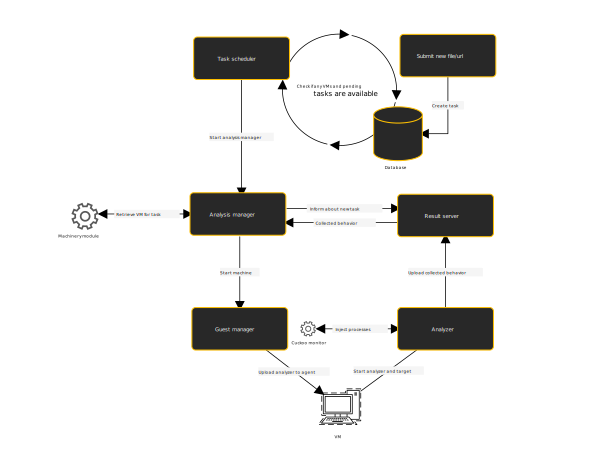
\includegraphics[width=8cm]{figures/flow.svg}
  \caption{\emph{CAPEv2} components and analysis flow (source \cite{CuckooSa10:online})}
  \label{fig:capeflow}
\end{figure}


\subsection{Network}
\emph{CAPEv2} provides multiple possibilities for \emph{guest} network setup which could be configured per analysis. 

In the case of \emph{None} routing, the machine is isolated. The only connection is the one with the result server. Additionally, there is \emph{Drop} routing when all the traffic is actively dropped (a more aggressive option). 

Other options provides internet connection (in some sense). \emph{Internet} routing is full internet access through specified interface. We can also forward the traffic through another gateway - \emph{VPN}, \emph{SOCKS5} proxy\footnote{example tool https://github.com/RicoVZ/socks5man} or \emph{Tor}\footnote{https://www.torproject.org/}. Last option is to use network simulation like \emph{INetSim}\footnote{https://www.inetsim.org/}.

\subsection{Other}
One of the crucial features of \emph{CAPEv2} is the debugger, so we can also perform non-interactive dynamic code analysis. It allows dynamic anti-evasion bypasses such as \emph{Guloader, Ursnif} or \emph{Zloader} uses.

\emph{CAPE} means \emph{Config And Payload Extraction}. The main motivation behind its creation was malware payload extraction, for which it uses techniques like Process injection, Decompression of executable modules in memory or extraction of executable modules. \emph{CAPEv2} automatically creates a process dump for each process that effectively detects basic packers.

It can detect various malware families such as Emotet, QakBot, Dridex and many others. It also uses Yara rules.

\subsection{Produced data}
The whole ouput of \emph{CAPEv2} is listed in the table \ref{tab:sandbox-out}. 

\begin{table}[h]
  \centering
  \caption{CAPEv2 Sandbox output}
  \begin{tabular}{p{2cm}p{6cm}p{6cm}} 
      \toprule
      \textbf{Output} &
      \textbf{Description} \\
      \midrule
      pcap report & network traffic record (packet sequences) \\
      \midrule
      memory dump & dump of RAM (its analysis results could be also presented) \\
      \midrule
      bingraph & mechanism that discovers metamorphic malware \cite{Kwon2012}\\
      \midrule
      behavioral log & raw logs of api calls and other (usually in \emph{BSON} format) \\
      \midrule
      dropped files & all dropped files unchanged in separate directory \\
      \midrule
      CAPE, procdump & other extracted payload in separate directory \\
      \midrule
      reports & JSON report and possibly other reports  \\
      \midrule
      screenshots & taken during analysis  \\
      \bottomrule
  \end{tabular}
  \label{tab:sandbox-out}
\end{table}


\subsubsection{Report}
As we stated in the thesis introduction, our goal is to use \emph{behavioural} features and \emph{signatures} from \emph{JSON} reports.  The most comprehensive report produced by \emph{CAPEv2} is in \emph{JSON} format. We will use this format as direct input for our model. Let us define this format \footnote{documentation https://www.json.org/json-en.html} and the content of the report.

JSON (JavaScript Object Notation) is a most frequently used lightweight data-interchange format. It consists of two essential structures - \emph{collections of key-value pairs} (sometimes called \emph{objects}) and \emph{ordered lists}. 

\emph{Object} is an unordered list of \emph{key-value} pairs, curly brackets surround it, pairs are coma-separated, and a colon separates keys from values. \emph{Keys} have to be double-quoted unicode strings. \emph{Values} might be strings, numbers, objects, arrays, boolean or null. \emph{Lists} are surrounded by square brackets and contains comma-separated values.

Usually, a single \emph{.json} file contains one object, but there are also cases where a list of objects is presented.

The \emph{CAPEv2} report usually has tens of megabytes but sometimes even gigabytes. Complete schema (list of attributes) of report is in \ref{tab:report}. In the thesis attachment, we can see an example of a real log (\ref{app:attach})

\begin{table}[h]
  \centering
  \caption{Parts of \emph{report.json}}
  \begin{tabular}{p{4cm}p{10cm}} 
      \toprule
      \textbf{Entry} &
      \textbf{Note} \\
      \midrule
      statistics & time statistics for particular part of malware analysis \\
      \midrule
      info & sandbox details (machine, category, used module, timeout\dots) \\
      \midrule
      debug & sandbox debug log \\
      \midrule
      target &  info about examined sample\\
      \midrule
      CAPE & extracted payload info \\
      \midrule
      behavior & processes, mutexes, commands and other behavioural attributes \\
      \midrule
      deduplicated shots & screenshot summary \\
      \midrule
      network & network traffic report (domains, tcp, udp\dots) \\
      \midrule
      static analysis & results per file \\
      \midrule
      strings & extracted strings \\
      \midrule
      suricata &  output of suricata network detection tool (\url{https://suricata.readthedocs.io/en/latest/quickstart.html})\\
      \midrule
      malfamily tag &  malware family detection result\\
      \midrule
      malscore &  malicious score\\
      \midrule
      signatures &  list of signatures detected by sandbox \\
      \bottomrule
  \end{tabular}
  \label{tab:report}
\end{table}

\section{Prior arts}
Below we list relevant publications where authors applied machine learning algorithm using the data produced by malware analysis tools.
\subsubsection{Static features}
\begin{itemize}
  \item Strings - \cite{Lee2011}
  \item N-grams (an analysis using bytes subsequences of length $N$ from original binary) - \cite{Fuyong2017}
  \item Entropy of the malware file - \cite{Wojnowicz2018}
  \item Statically extracted API functions calls - \cite{Ahmadi2016}
\end{itemize}

\subsubsection{Dynamic features}
\begin{itemize}
  \item Registry - \cite{Ghiasi2015}
  \item CPU instruction traces - \cite{Carlin2017}
  \item Network traffic - \cite{Boukhtouta2015}
  \item API call traces -  \cite{Galal2015}
\end{itemize}

Other related resources might be \cite{Singh2020, Sethi2019, Abdessadki2019, Gibert2020}.


This chapter described the essential background of malware, its analysis, and specifically \emph{CAPEv2} sandbox and its output. 


%%------------------------------------------
% Let us summarize basics of malware interaction with windows OS (main source \cite{Sikorski2012}). nice to have chapter ANALYZING MALICIOUS
% WINDOWS PROGRAMS
% Types, Families
% https://en.wikipedia.org/wiki/Malware
% Find in books!
% https://www.sciencedirect.com/science/article/pii/S1084804519303868 - good overview and taxonomy of malware


% \todo{describe part one goal - We involve more theory and prior work research, in following chapters we discuss our case.}
% In the first part of this thesis we focus the comprehensive theory which is needed to absorb in order to interpret results. Not everything is disassembled in detail we go only there where we find something useful for our thesis. This is really based on experience so if the reader is interested only in results used formalism and notation in theory part are important only.

% \todo{Summarise what we know from previous sections \todo{especially from analysis part, where we should summarise what usual program is doing in the computer and what we can observe (and what we can get from cuckoo monitor)} and go to the most concetrated information about run of program - we should end at the things which are in summary part of json log, but we can have more variants}



% Last remarkable not is many times analyzed statistical assumption
% My
% Data quality, bias, antisandbox detection... where to find samples? (we should definitely mention motivation why we are collecting our own data), public data (this is quite risky to publish in general), everything is fast (zero days), Are those anomalies or malicious?, Imbalanced data sets, encryption everywhere - what to trust..., cryptocurrencies, iot, cloud

% \todo{add some motivation example or latest results... - known malware attacks..}

% Philosophy could be walking around risk management, probability of risk and resulting damage... Maybe more examples of situations where we know how much it cost (Cambridge analytica, ransomware...)
% Maybe something about truth and its protection in the world of lies and fake news
% Confidentiality, integrity and availability

% Use found books or post-hoc go through some articles and formulate the motivation part...



% Nice to have
% https://github.com/kevoreilly/CAPEv2/blob/master/changelog.md
% http://docplayer.net/62887099-Cuckoo-malware-analysis.html
% https://cuckoo-monitor.readthedocs.io/en/latest/hooks.html, more comprehensive description of cape monitor
% Processing modules

% existing solutions and results...
% find basics in books

% api hooking, dumping import reconstruction debugging static parsing - https://www.youtube.com/watch?v=qEwBGGgWgOM

% to appendix we can add also web interface of cuckoo
% \section{Prior}
% works about malware analysis
% works that collected data for machine learning purposes
% Mandlik, Stiborek, everybody who used cuckoo or other sandbox data (reference for what and their results)

% file:///C:/Users/domia/Downloads/Imad-Saiida-IJCNIS-V11-N6-1.pdf
% https://web.archive.org/web/20160418151823/http://www.ijarcsse.com/docs/papers/Volume_3/4_April2013/V3I4-0371.pdf
% https://reader.elsevier.com/reader/sd/pii/S1383762120301442?token=81F1AB06FF0FE40D1B7745234269280FCF2CB0979140E84DB35D6E04A2C622FE6EDA2DE4DA0630E1D73044E3D84A722F&originRegion=eu-west-1&originCreation=20210401090943
% https://iopscience.iop.org/article/10.1088/1742-6596/1140/1/012042/pdf
% file:///C:/Users/domia/Downloads/JCIT4024PPL.pdf
% https://dl.acm.org/doi/abs/10.1145/2046614.2046618?casa_token=MXpfHiylCZcAAAAA:szRMPWfKXTl4wxP2-h32eknCg5dzM2t7RxGjywiJDksmT5FqcUY7pPrIBZchv26HUe3Lwubu5Hru

% file:///C:/Users/domia/Downloads/088851962.pdf

% mention signatures
% usual format which are produced by sandbox and what we can find there
% Reference even docs - no problem, not only books and papers
% Conclusion should be that those data are complicated and their structure also keep some information (order, structure...), that is why we want to focus on structured data and especially json.
% size...


% TODO - nice-to-have
% memory forensics


% If I have to add something - https://publications.sba-research.org/publications/malware_survey.pdf



% mention especially parts which gives more information about the run (mutexes, files, api calls,.. - to be able to reference from data chapter)

% - Summary of potential sorces of metadata
% ○ Abuse.ch - https://bazaar.abuse.ch/api/#api_key
% ○ VirusTotal - https://developers.virustotal.com/v3.0/reference#file-info
% ○ Metadefender - https://onlinehelp.opswat.com/mdcloud/3.1_Retrieving_scan_reports_using_a_data_hash.html
% - Interesting



% Previous connection
% - Nothing before
% Way through this chapter
% - Malware definition and types
% - Malware analysis
% - Challenges
% - Data - input, output...
% - prior
% Next connection
% - We are interested in modeling the data using modern approaches, we know that the data are often structured somehow and that is what we will solve

% - GOALS
%   - Run several instances of CapeV2 sandbox and solve their orchestration for this experiment
%   - Capture behavior of selected malware samples in CapeV2 sandbox and store results
% - Theory part - types, conditions, bias, Malware types, signatures....
% - Sandboxing
% - Previous experiments
% - Our goal in this part
% - Data collection for ML purposes in general


% https://www.groundai.com/project/machine-learning-in-cyber-security-problems-challenges-and-data-sets/1

% https://www.readitquik.com/articles/security-2/cybersecurity-challenges-that-need-to-be-on-your-radar-right-now/
	%\chapter{Malware classification}
We can expose a lot of information from malware analysis result. It contains api calls, network requests, downloaded payload and much more. This could be used to explain directly what is going on during the run. Sandbox itself is often labelling malware samples using so called signatures. These signatures are deterministically assigned and they usually sign that particular malware sample is doing something suspicious (we will describe later). Based on signatures we can later distinguish between different kinds of malware or between malware and cleanware - classify. Besides this deterministic way modern approaches from machine learning are often used.

In this chapter we focus on classification problem in general and later we describe malware classification. We involve more theory and prior work research, in following chapters we discuss our case.

In previous chapter we described different data outputs which are often produces by different kinds of analysis. That why later in this chapter we focus on models which are designed to for such data.

\section{Classification in general}
\todo{Add some examples of use of ML and AI in cyber security field}


\todo{I think we want to aim only on stastistical machine learning, so let's define it at the beginning}
The largest challenge in machine learning theory is very often used formalism and framework and point of view which we consider. So firstly we would like to summarize where in this tangle we are and where we are going.

As stated by \citet{GoodBengCour16} the usual aproach in distinguishing tasks for machine learning algorithms are most often divided in categories based on expected sample processing result. By sample we mean collection of features which tends to be represented as $$TODO: add vector on R or tensor on R$$. As an example we can introduce images with fixed dimension but in our usecase even serialized json files or pcap files.

In this section we are aiming at standard machine learning approach and tasks formulation, later we will define task which is actual for our work.

\todo{add scheme of machine learning algorithm in classical manner, so features to hidden states (sometimes label) mapping, define some formalism for math signing}

\paragraph{Usual and most seen categories are:}
\begin{enumerate}
    \item Classfication \todo{describe, add some math}
    \item Regression \todo{describe, add some math}
\end{enumerate}

There are other categories like transcription \cite{GoodBengCour16} or anomaly detection \cite{Chandola2009} which is quite often seen in cyber security field \todo{add example of this kind of task in cyber security https://link.springer.com/article/10.1007/s10994-014-5473-9}. And many other defined problems mentioned in \cite{GoodBengCour16} or \cite{zhang2020dive}.

Based on presence of hidden states and other conditions we can further distinguish between supervised and unsupervised learning tasks. \cite{zhang2020dive}. One of the biggest challenges of machine learning nowadays are labelled data, where every sample consists of features and appropriate hidden state - dataset for supervised learning. That is one reason why we want to be able to face even situations where the hidden states are not presented - dataset for unsupervised learning. \todo{add some paper where they talk about challenges like this} Those situations we can very often see in cyber security field because in principle attacker or any kind of distractor often wants to hide acts such that protector is not able to identify. So the hidden state itself could be assigned rather based on further data collection or never.\todo{find something about unsupervised learning in cyber security as an example https://technative.io/why-unsupervised-machine-learning-is-the-future-of-cybersecurity/, https://ieeexplore.ieee.org/abstract/document/8268746?casa_token=ctNKO2pD640AAAAA:XoFuD8SHvbzMszA1nHciHIiaetBCG7fN47zUNZDMYv2D5oZUqhGuq9FF_ETI9Rhf7QtsTYagkw, https://arxiv.org/abs/1812.07858}.
There are also cases where we talk about semi-supervised learning \todo{define it and reference some source for example GoodBeng is mentioning it}.

\todo{from this we can go to missing values in data and maybe even to various dimesion data learning}

The oposite point of view on non-ideal datasets are those where features are missing. \todo{http://www.iiis.org/CDs2008/CD2008SCI/SCI2008/PapersPdf/S507DT.pdf is source of information here}

Later we will mention other examples of tasks mainly different in the assumtions for input data.

\todo{Here we can find something else https://machinelearningmastery.com/a-tour-of-machine-learning-algorithms/}

Our task is to classify samples so in further writing as model we reference classification model.

train, test, validation and hyperparameters, overfitting, underfitting (https://www.deeplearningbook.org/contents/ml.html)


\section{Classification models}
There are various approaches to classification. In this section we describe some of basic models and their usual output and its intepretation. 

reference discriminative models because this paper is talking about it also - https://dl.acm.org/doi/pdf/10.1145/2996758.2996761 and we will work with that in further sections

Mention on what kind of optimization it stands
https://analyticsindiamag.com/7-types-classification-algorithms/
https://www.edureka.co/blog/classification-algorithms/#typesofclassificationalgorithms
https://dzone.com/articles/introduction-to-classification-algorithms

\section{Model Evaluation}
Based on what we are solving and what we want to comapare to we have to choose proper metrics to evaluate our classifier. Majority of those techniques does not depend on type of classifier we have. The classifier itself is just blackbox which we are evaluating based on simply classificcation results.
Mention training and learning case and metrics in different context
general measures
nice-to-have: early stopping based on metrics like those
https://www.researchgate.net/profile/Mohammad-Hossin/publication/275224157_A_Review_on_Evaluation_Metrics_for_Data_Classification_Evaluations/links/57b2c95008ae95f9d8f6154f/A-Review-on-Evaluation-Metrics-for-Data-Classification-Evaluations.pdf

measures important in cyber security
https://scholarcommons.usf.edu/cgi/viewcontent.cgi?article=1005&context=mca
https://ntnuopen.ntnu.no/ntnu-xmlui/bitstream/handle/11250/2730527/Hameed%252C%2BIbr.pdf?sequence=2&isAllowed=y
https://owasp.org/www-community/controls/Intrusion_Detection
On the other hand I will write even my own reasoning in particular in domain of cyber security what does it mean to misclassify as positive or negative example...
In majority of papers like this https://core.ac.uk/download/pdf/77064684.pdf, they just state what they use fo accuracy and done. Or here :D https://core.ac.uk/download/pdf/80994982.pdf
this is aiming at false positives in cyber security https://ieeexplore.ieee.org/document/7560382
Goal obviously is to keep high false negative and lowen false positive beacuse both metrics are really important in network security
https://www.ccdcoe.org/uploads/2018/10/Art-19-On-the-Effectiveness-of-Machine-and-Deep-Learning-for-Cyber-Security.pdf - section fn and fp



\section{Data characteristics}
Model which we choose for given task is based on several facts like domain which we are dealing with and mainly on the data we have.
Input to usual model is binary vector or rather tensor, but those tensor could be encoding of different things
Basic point of view is to distinguish between two basic types of variables - continous and discrete (https://machinelearningmastery.com/feature-selection-with-real-and-categorical-data/)
Highlevel view will refer to images, time series, graphs (json...), just binary...
Maybe we can talk about fixed dimension, various dimension

Write more about json files and generally describe graph inputs

\section{Neural Nets}
In the section models \todo{reference} we briefly described different kinds of models. One specific model we would like to discuss more copmrehensively - neural nets. The reason is that our method is building on top of this approach.

Neural nets are machine learning phenomenon mainly because its robustness and not so demanding data assumptions. \todo{examples of use and some reference to this statement, https://stats.stackexchange.com/questions/467103/do-neural-networks-make-assumptions-about-data-and-when-to-use-standardization}.
general even math!
https://www.deeplearningbook.org/contents/ml.html
http://neuralnetworksanddeeplearning.com/chap1.html
http://playground.tensorflow.org/#activation=relu&batchSize=30&dataset=spiral&regDataset=reg-plane&learningRate=0.3&regularizationRate=0&noise=0&networkShape=4,2&seed=0.87951&showTestData=false&discretize=false&percTrainData=50&x=true&y=true&xTimesY=false&xSquared=false&ySquared=false&cosX=false&sinX=false&cosY=false&sinY=false&collectStats=false&problem=classification&initZero=false&hideText=false

optimization theory, gradient descent, stochastic gradient descent, backprop
cs.huji.ac.il/~shais/UnderstandingMachineLearning/understanding-machine-learning-theory-algorithms.pdf
https://stats.stackexchange.com/questions/186091/what-loss-function-should-i-use-for-binary-detection-in-face-non-face-detection

Loss functions and nets used for classification
https://machinelearningmastery.com/how-to-choose-loss-functions-when-training-deep-learning-neural-networks/

\section{Classifying based on graph structured data}
Real world use cases provide often more complex dastasets than just fixed dimension matrices or images. As we mentioned our data are often stored as JSON files. Those files could be formally seen as tree-structured inputs for machine learning algorithms. 
\subsection{Problem}
https://www.quora.com/What-is-structured-data-in-the-context-of-machine-learning

https://www.naftaliharris.com/blog/machine-learning-json/

\subsection{Prior}
https://arxiv.org/pdf/1506.05163.pdf
https://arxiv.org/pdf/1911.08756v3.pdf
https://www.cs.uoregon.edu/Reports/AREA-201706-Riazi.pdf
https://core.ac.uk/download/pdf/11011889.pdf
Hmill
Graphical models
Graph neural networks
    Also seen here file:///C:/Users/domia/Downloads/Explainability_ICML2021.pdf
See in Mandlik

\section{Classification in cyber security, classifying malwawre}
file:///C:/Users/domia/Downloads/CoRR2018_submission_v3.pdf
https://www.sciencedirect.com/science/article/pii/S1084804519303868
Finally we can not skip our domain and results in this field. 
Kinds of classifications in cyber security and their description
Intrusion detection, network traffic attacks and anomalies and malware X cleanware classification,...
We can classify different things like malware X cleanware, malware family (not so useful in detection but in further learning)
Problems of cyber security field
Based on Dynamic, static, other kind of input data...
SURELY MENTION RETRAIN PROBLEM AND reason that this is true but machine learning algorithm could be much more efficient (this is kind of motivation of our work)
https://www.ccdcoe.org/uploads/2018/10/Art-19-On-the-Effectiveness-of-Machine-and-Deep-Learning-for-Cyber-Security.pdf (eventually their references - some interesting research results, good for prior)
https://www.groundai.com/project/machine-learning-in-cyber-security-problems-challenges-and-data-sets/1
https://arxiv.org/pdf/1910.11376.pdf

If I finally go through this summary report I will be save with this part hopefully - https://www.jstor.org/stable/resrep22692?seq=53#metadata_info_tab_contents, this is great summary for modern approaches and papers in cybersec, I can use it even somewhere else for example in intro of this chapter and whole thesis
For example one part was focused on types of classifiers - in machine learning is quite big difference between zero-days and known malware...

Using N-grams in detection https://www.researchgate.net/publication/262366662_A_Close_Look_on_n_-Grams_in_Intrusion_Detection_Anomaly_Detection_vs_Classification

Malware classification in more detail

not so interesting can be added between other examples - https://www.researchgate.net/publication/312964059_Malware_Classification_Based_on_Dynamic_Behavior, https://link.springer.com/content/pdf/10.1631/FITEE.1601325.pdf, https://dspace.cvut.cz/bitstream/handle/10467/87850/F3-DP-2020-Dvorak-Stepan-dvorast6.pdf?sequence=-1&isAllowed=y (mention graph neural networks)

Using static analysis https://dl.acm.org/doi/pdf/10.1145/2402599.2402604?casa_token=Kv3xJb3iPssAAAAA:rm6bhWnusg7eEvalXNveaJXILphAxhpZHGS6OxpDk36na4q5u9RpZ3gM83IMQWq1QQ0aEIVoeyZN

family classification - https://arxiv.org/pdf/1912.11249v1.pdf

Recurrent networks - https://ieeexplore.ieee.org/stamp/stamp.jsp?tp=&arnumber=7178304

HMILL in cyber security - https://arxiv.org/pdf/2002.04059.pdf, mandlik, Pevny

\subsection{Problem}
\subsection{Prior}


\todo{add conclusion of this chapter and connection to next chapter - hmill}




Previous connection
- One of conclusions of previous chapter is that that character of data is often structural as graph or tree (json, xml,...)
Way through this chapter
- Generally about machine learning challenges and types of tasks
- Classification models and their evaluation
- Neural networks
- Classifying structured data as jsons - models
    - hmill and other techniques - reference next chapter
- classification task in cyber security
- Prior on this topic - cyber security!
Next connection
- Hmill is one what we want to use to create model of the data for classification


\cite{GoodBengCour16}
Potentially:
- general points at the beggining
    - Increasing model sizes
    - Increasing Accuracy, Complexity and Real-World Impact
    - Gradient-Based Optimization
    - Stochastic Gradient Descent
    - Challenges Motivating Deep Learning
- More Sure
    - Supervised X Unsupervised
    - The Task, T - classification, regression, others exists
    - The Performance Measure, P
    - Capacity, Overfitting and Underfitting
    - Hyperparameters and Validation Sets
    - Bias and variance - Trading off Bias and Variance to Minimize Mean Squared
    Error

\cite{Bishop2006}
 - generally the introduction to classification models


- Classification problems - binary, multiclass, multilabel...
- Theory
- Single label, multilabel

- evaluation of classifiers - more or less independent on model choose
  - Confusion matrix
  - F-score, train accuracy, test accuracy, loss function, plots
        - AUC, ROC?
  - What is important metric during malware classification and why


- learning classifier from graph data - json files,...
- possible models - based mainly on the data structure we have and use case we are modelling (find how to choose proper model)
    - among them even neural networks and refer to mill/hmil in next chapter - connect to goal of this thesis, use this framework to classify malware - go on with next part
- (one of them should be using neural nets - describe deeply usage of loss function in both cases - single label, multi label...)
- hyper parameters...
- minibatch gradient descent, gradient descent itself

- Machine learning in cyber security in general
- General approaches to malware classfication - theory
    - classifying type of malware or some kind of behavior X classifying malware Vs. cleanware
    - based on dynamic/static anysis results...
    - get to neural network and finally to mill - stiborek and other applications in cyber security (Mandlik, Pevny, Dedic...) and reference next chapter.


- Prior work
Our goal is not to compare, mentions are just for reference to similar work, mention practical papers used above

nice-to have:
- (Overfitting, early stopping)

Remainders:
Malware analysis results could be used
Following data collection and processing next task is  
Based on type of analysis and characteristics of collected data}

	% \chapter{Hierarchical Multiple Instance learning}
The goal of this thesis is to use specifically hmill learning to classify malware samples. Using it we want to  build on the prior work in this area. \todo{add references}

In this chapter we describe Hmill framework and use cases where this kind of learning was involved. Then we will address its usage in malware classification and other applications in cyber security field.


Stand on Madlik chapter, his citations (be aware), somol and Pevny

Previous connection
- We focus on structured data and our tool is hmill, let's describe it
Way through this chapter
- multiple instance learning
- hierarchical mill
- prior
Next connection
- Not necessary, but can connect to next chapter slightly (we want to explain this kind of model)




- GOALS 
- Learn the hierarchical multiple instance learning framework (HMill)
- describe theory, connect it to classical approach
- Usual usage of this type of learning - classification, regression...
- Our usecase and experiments with this kind of learning in malware classification field (prior)
	% \chapter{Model explaining}


Previous connection
- Hmill models and their explanation
Way through this chapter
- Explaining in general
- Explaining mill and hmill
- Prior
Next connection
- Next should be little summary of first part of thesis


Start generally about explaining and then methods proposed by Pevny

	\part{Usecase and experiments}
	% \chapter{Infrastucture and data collection} \label{chap:infrastructure}
This chapter describes the realization of the data collection process using \emph{CAPEv2} sandbox. The sandbox is described in the chapter \ref{chap:analysis}, here we focus on the specific setup, problems we experienced and their solution. We have a data source of malware samples MalwareBazaar mentioned in the thesis introduction. The output of this task is a dataset of dynamic malware analyses. It includes behavioural features and signatures, both input for our \emph{HMill} model.

Although this chapter is shorter than the previous ones, we spent the most significant time on this task. All scripts and other outcomes are part of the attachment (\ref{app:attach}), and the most important tools are listed in \ref{app:technologies}.

\section{Host machine}
The host machine is where the sandbox environment and virtualization software is running. We know that an analysis of one malware sample takes up to five minutes, and we want to have as many samples as possible. That is why we want to run several distributed host machines. 

The whole process of a host machine initialization is automated to be able to set it up multiple times. The initialization consists of several steps:
\begin{itemize}
    \itemsep0em 
    \item Install host operating system --- recommended Ubuntu
    \item Enable SSH to be able to access it remotely
    \item Enable basic security --- firewall and supporting tools
    \item Install virtualization software --- recommended KVM QEMU
    \item Copy virtual machine images to the host
    \item Sandbox initialization and configuration
    \item Data collection script initialization
\end{itemize}

To run all steps on multiple machines at once, we used Ansible, a network orchestration tool. We also added some usual management functions, e.g., to copy new configurations from the server or clean up the sandbox data.

Hardware resources on host machines are 256GB SSD and 16GB RAM, which means that a sufficient number of virtual machines per one host is four. We experimented with more, but there was an overload which might lead to biased analysis results.

Various issues accompanied the automation of the whole process. Such a process often needs manual steps, and their automation is very challenging. Issues were caused mainly by our low experience, and sometimes poor documentation was involved. Especially the process of virtual machine images creation and copying was connected with issues. Overall, we have configured seven host machines.

\section{Guest machine}
Guest denotes the virtual machine where the malware sample runs and where the \emph{CAPEv2} monitor operates. We used Windows 7 as an operating system. The crucial goal of the guest machine is to look like an ordinary computer that is in regular use. Due to the virtualization usage, we had to care about the sandbox evasion techniques mentioned in \ref{chap:analysis}.

There are two options for anti-evasion setup in \emph{CAPEv2} sandbox. Firstly, we experimented with vmcloak\footnote{https://github.com/hatching/vmcloak}. We were able to run and use this tool. However, it supports only VirtualBox, which is not recommended by \emph{CAPEv2} because of its performance. The project is also no longer maintained, and some functions did not work, e.g., taking snapshots. The second option is to use a script recommended by sandbox contributors\footnote{https://github.com/doomedraven/Tools/blob/master/Virtualization/kvm-qemu.sh} and perform manual steps in the virtual machine configuration\footnote{https://www.doomedraven.com/2016/05/kvm.html\#modifying-kvm-qemu-kvm-settings-for-malware-analysis}. After several unsuccessful attempts with low-level virtual machine misconfigurations, we were able to create four working images.

The sandbox requires disabling the firewall and running Python on the guest machine. We added the most popular applications like Google Chrome, Firefox, Adobe reader, Spotify. We added one private key to C://Users/Administrator/.ssh and one password to the Google Chrome password database. We downloaded random images and documents from the internet.

\section{Network setup}
The network setup is a crucial point in the dynamic analysis. The guest machine has to reach the host machine to stay in touch with the result server. Secondly, there is an internet connection for the guest, which might be necessary for some malware types. As an example, we can see \emph{dropper}, which is responsible for downloading a payload.

We decided to collect the data under two different conditions --- with an internet connection (denoted by \emph{internet}) and without (denoted by \emph{none}). We engaged both because the \emph{internet} is much more difficult to set up and secure, and we wanted to start data collection as soon as possible. Both architectures are figured in the appendix \ref{app:network}.

\subsection{None}
\emph{None} setup is a straightforward option for an isolated network between host and guest. This approach requires a host-only interface created in \emph{KVM} virtualization tool. Host and guest are assigned with IP addresses from the same range. From a security point of view, we have to set up a firewall on the host machine. It should accept connections from the isolated network only on the result server's port.

\subsection{Internet}
We want to provide internet access to the guest machine during the analysis run. For this purpose, we prepared a VPN connection to the secured network through which the communication should be forwarded. That is considered a good practice to observe what the samples are doing and be able to stop it fastly. We call this network \emph{dirty lab}.

\emph{CAPEv2} supports VPN connection setup for each guest machine separately. We knew that it would be better to have a central gateway for all local traffic than connecting each particular guest machines to the \emph{dirty lab}. However, we decided to use native sandbox functions at first. After experiencing some issues with \emph{CAPEv2} VPN configuration and an unsuccessful issue reporting, we decided to find another custom way. 

The main requirement is to centralize the traffic from the local network (malicious) to \emph{dirty lab}. The exit point we call \emph{router}. The surrounding university network has to be secured and isolated from malicious traffic. We also need to monitor host machines because of a potential intrusion and centralize logs from host machines.

In the following text we use \emph{l2} and \emph{l3} as a designation referring to ISO/OSI model of network communication \cite{Zimmermann1980}. By \emph{l2} we mean communication on the data link layer. Specifically, we mean ethernet/802.11 local networks where MAC (Media access address) is used for device identification. By \emph{l3} we mean IP communication on the network layer. IP addresses are used for device identification on \emph{l3}.

An expert recommended the designed network architecture after a consultation. Its basic idea is to avoid \emph{l3} communication on the local network such that IP address from one range is assigned only to the guest machine and then to the router device. This idea was supported mainly by the \emph{l2} VPN on the local network.

The role of the router is to receive the traffic going out of the local network and forward it to the \emph{dirty lab}. It can also monitor and capture the traffic. In \emph{dirty lab}, we were provided with the ipv4 interface only, so the \emph{router} performs network address translation (NAT). \emph{Router} machine is running Ubuntu operating system. It is configured to connect to \emph{dirty lab} using \emph{l3} VPN and to the guest machines using \emph{l2} VPN. In \emph{l2} VPN, \emph{router} is a server and in \emph{l3} VPN, it is a client (server is running in the \emph{dirty lab}). \emph{Router} is realized as a virtual machine with fast recovery capability. All logs from the server are sent to the central machine.

The host machine has to be configured as a client in communication with \emph{router} using \emph{l2} VPN to forward the guest's traffic through it. The idea of this setup is that all the traffic leaving this device is encapsulated in packets with university network IP addresses. This network is unknown to the guest device where malware is running. From the guest's point of view, the connection between the \emph{router} and a \emph{guest} is on \emph{l2}. 

On the host, the interface for \emph{l2} VPN communication (TAP) is bridged with the original interface, which allows communication with the guest virtual machine (originally host-only). 

A connection to the internet from the guest machine goes through the host machine, the router, and the dirty lab to the internet. 

There has to be an additional setup on the host machine besides that listed in the case of \emph{none}. Each host machine in the distributed cluster has to send all sandbox logs to the central Syslog server. All machines have to be set up with a monitoring tool to detect intrusion\footnote{example https://aide.github.io/}.

\section{Data collection pipeline}
During the distributed data collection, we used the following terminology. \emph{Master} is a machine responsible for sample distribution, and it has access to a NAS, where it stores analysis results. \emph{Worker} is another name for \emph{host} machine in the context of distribution.

This section describes the whole process of data collection, beginning with a malware sample going over its dynamic analysis and ending with the behavioural features and signatures extracted from the \emph{JSON} report. All programs implemented to solve the mentioned problems are part of the attachment (\ref{app:attach}). Particular steps are automated, and their description follows.

\begin{enumerate}
    \itemsep0em 
    \item Download samples from the \emph{malwareBazaar}
    \item Filter PE files only
    \item Retrieve additional metadata
    \item Add hashes to database
    \item Distribute samples to workers
    \item Analyze samples and send results back
    \item Store results
    \item Extract JSON reports
    \item Prune unnecessary parts
\end{enumerate}


\subsection{Abuse.ch MalwareBazaar}
The place where we downloaded malware samples was abuse.ch\footnote{https://abuse.ch/} specifically part called \emph{Malwarebazaar}. The reason for its usage is free access without any claims. \emph{MalwareBazaar} is a database of malicious (no benign files or adware) samples that anybody can share and download. In May of 2021, it contains over 325~000 samples. Malware samples are downloaded in the compressed form --- one archive for every day since the start of the \emph{MalwareBazaar} project.

\subsection{File filtering}
Our project aims only at PE files described in \ref{chap:analysis}. After decompression of the original archives, we filter the files based on the file extension and file headers. We also filter the compressed files, decompress them, and again filter PE files only.

\subsection{Metadata}
The secondary intention was to obtain some basic metadata about each file to have basic information. We were able to gain academic access to the VirusTotal API\footnote{https://developers.virustotal.com/v3.0/reference}. We downloaded a metadata report for each of our samples. The report contains basic static information like hashes and fuzzy hashes, extracted strings, detection of various antiviruses, and even a summary of reports of used sandboxes.

\subsection{Distributed sandbox}
After dealing with issues in the host initialization part and even in the VPN setup part, we also encountered issues while setting up the distributed sandbox. \emph{CAPEv2} can orchestrate multiple host machines. It uses distributed mongo database\footnote{https://www.mongodb.com/} combined with a script that is run on the master machine to check the connection to the registered worker devices. We spent with the configuration of distributed \emph{CAPEv2} large amount of time trying multiple different ways and following several pieces of advice but unsuccessfully. We decided to implement our lightweight solution for time reasons.

Hashes of our files are stored in a database (in our case \emph{JSON} file) with additional attributes. A script runs on the master machine that distributes samples among worker machines using their REST API. After the analysis is done, another script on the worker machine compresses the result and sends it back to the master. The last script manages the coming results and saves them to the NAS. Everything is recorded in the database.

\subsection{Result postprocessing}
We need only part of the \emph{JSON} report, specifically behavioural features and signatures, for further modelling. Its extraction was done in two steps. Firstly, we decompressed the analysis result and extracted the \emph{JSON} report only. Secondly, we extracted the mentioned parts and saved the shrank output. The whole report might have even gigabytes. However, the shrank variant has usually tens of megabytes. We could transfer the output to the metacentre where the model computation and explanation took place.

\section{Collected dataset}
When we start modelling experiments, we have a dataset consisting of 80,000 different samples in \emph{none} network setup. The \emph{internet} configuration took us several weeks to deal with, and the data collection started later and was slower. The \emph{internet} data will be investigated in future work as its collection continues. 

The complete dataset has approximately 2,5~TB in compressed form. Extracted features and signatures are much smaller (tens of gigabytes). 

Not all outputs of the sandbox described in \ref{chap:analysis} are presented in each analysis result because the configuration and other conditions influence it.

After examining the histogram of seen signatures, we chose a subset based on their frequency in the training set. We prefered signatures that are implemented in Python for convenient investigation of the original cause. In \ref{app:signatures}, our candidates can be seen --- their frequencies in the dataset, and additional information, including even the groups described in the chapter \ref{chap:classification}.
	%\chapter{Data structure, features and hidden states}


Previous connection
- Follow up statements about data in cybersecurity, follow prevous chapter with choosing relevant parts of logs
Way through this chapter
TODO
Next connection
- Chosen data will be used for further experiments



reference json grinder and its usage to process data

reference some source that is talking about data in cyber security, resp. on theory part

- What kind of data we have - mention all parts of cuckoo log, mention even virus total reports
- (theory for basic statistcs, but maybe not)
- GOALS
  - data processing, pruning and so on
  - Analyze captured data. Report basic statistics and choose appropriate features and hidden states for further modelling
- dataset structure
  - Bias in practical data like this - security data, what are the influences
  - Balanced dataset - in term of accuracy metric performance
  - What each part means (including signatures)
- basic statistics - histogram...
- On Hmill usage - features, hidden states (Section for each, description)
- Signatures - hidden states
- Features  desription
- Maybe try to extract more candidates (But I would have to perform several more experiments, but data pruning should not be problem)
  - I tried to choose enhanced and summary part but it was too much and enhanced part contains bias like timestamp and so on, so I decided to choose only summary part and later only segments from it, using whole summary lead us to really slow convergence...I think

	%\chapter{Modelling classifier}
Following previous chapter we want to present our way of modelling and results we have. The main goal of this part is to train the models based on prior experiments, not strictly perform long sequence of experiments and compare to prior. On the other hand we would like to present similar metrics comparing to our colleges. We did not model all variants mentioned in previous chapter, we concentrated on at least one working model and then we move on to model explaining experiments.

In previous chapter we formulated several possibilities for model output and input. We use \emph{hmill} framework for data modelling \todo{reference hmill chapter}. From \emph{states} and \emph{features} in question we started with our top candidate - \emph{signatures} as states and \emph{behavior log} as features. Our reasoning is based on the fact that the signatures are assigned based on some usually atomic fact, for example presence of some api call in log. If we choose part of behavior log where this information is presented, we should be able to evaluate model's prediction. Also we want to see if the model is able to generalize the knowledge and maybe come up with some new explanation of particular signature or just things which go with the original subject of particular signature. More complex labels like malware family or malware score are something what we can explore later. We assume that the assignement of those is often supported by signatures themselves and it should be better to explore the original cause of the whole chain.

\section{Behavior as feature vector}
After further look at the \emph{behavior} part of \emph{report.json} we start with only \emph{summary} and \emph{enhanced} part. The reason is that other parts are quite comprehensive and we will not be able to train the model. \todo{some better arguments}. If the model would be still to complex to train in our conditions we omit also the \emph{enhanced part}.

\section{Signatures as labels}
Brief description of signatures is in previous chapter \todo{ref chapter data}. Signatures are assigned to each sample based on its behavior. In figure \todo{add histogram visualization with percentage, not exact numbers} There is a histogram where we can observe frequency of each signature in our dataset.

From the original histogram we have chosen most seen signatures starting with \emph{injection_rwx} (because \emph{dynamic_funciton_loading} is almost everywhere). In the figure \todo{add table of resulting signatures or another pie graph} we can see our candidates. 
Next task is to try to investigate what the implementation of particular signature is about and try to create groups for further conclusion making. \emph{Python} implementation of each signture is processing the output of sandbox and generates boolean values signing that the subject of particular signature is presented in sample behavioral log. Subject of the signature can be api calls, dropped files, processes, commands and even something more complex. If the signature implementation returns \emph{True}, we observe instance of this signature in the \emph{signatures} part of \emph{report.json}. The format is following: \todo{add signature structure with example}

We explored two types of grouping aspects. First is the subject of particular signature and then second is if we can see this subject in the behavioral log directly. For instance if the signature implementation is using api calls so the api call list is directly in the log. If it uses entrophy of dropped files, it is not directly in the output. In figures \todo{add example of signature implementation}. Based on those criteria we identified following categories:
\begin{enumerate}
  \item Directly in \emph{report.json} in part \emph{summary, enhanced}
  \begin{itemize}
    \item API calls
    \begin{itemize}
      \item injection_rwx
      \item antidebug_setunhandledexceptionfilter
      \item removes_zoneid_ads
      \item deletes_self
      \item stealth_timeout
      \item enumerates_running_processes
      \item injection_runpe
    \end{itemize}
    \item Files
    \begin{itemize}
      \item copies_self
    \end{itemize}
    \item Commands
    \begin{itemize}
      \item uses_windows_utilities
    \end{itemize}
  \end{itemize}   
  \item Not directly in \emph{report.json} in part \emph{summary, enhanced} (it does not matter that no clues can not be there, but just not directly the information is not there)
  \begin{itemize}
    \item Processes - \emph{dropper}
    \item Sleep - \emph{ antisandbox_sleep}
    \item Entrophy - \emph{packer_entropy}
    \item Combinations - \emph{stealth_network}
    \item authsign - \emph{invalid_authenticode_signature}
  \end{itemize}
\end{enumerate}
\todo{add the data below without the frequencies to the structure}
More detail about each signature is in appendix \todo{add appendix where each signature will by summarized, its implementation and its data part...}

The reason why we categorize the signature in such manner is that we would like to connect those categories with the model performace in the further discussion.

\section{Model}
Describe mathematically what are features and labels and that we perform binary classification. Mention multilabel just marginally.
mention even multilabel as addition (in principle it should be possible but for us it was not priority)

\section{Modelling experiments}
Technology stack we used to train \emph{hmill} model is described in \todo{reference the appendix}. Important is that we unsuccesfuly experimented with multithreading in \emph{Julia} so the resulting model was trained only on one CPU.

First experiments are without reported results because model was to huge to converge, we were not able to train it on hardware we had and with thread limitations. This reality led us to skip one part of feature vector - \emph{enhanced} part. So the resulting model is working with \emph{summary} of original report only. \todo{clarify this in section introductions and so, not to confuse somebody with those ongoing changes}.

Original code of the model is in appendix \todo{reference appendix}. The pseudocode of the whole process can be seen on \todo{add pseudocode of analyser.jl}. It is obviously standard binary classifier. What is not so ordinary is that the model is function of the input data (typical for \emph{hmill}). Other interesting fact is that the \emph{hmill} framework API is more general so its is not accepting json documents directly. For this purpose we use \emph{JsonGrinder} library \todo{reference technology stack, where we describe the library a little bit and reference} which is able to accept array of json documents and produce schema \todo{add this schema and extractor to appendix exported} which is then used to create \emph{hmill} object from each json document.

\subsection{Model hyperparameters and dataset attributes}
In our experiment we do not involve techniques like early stopping or hyperparameter tuning. We build on previous experiments namely on \cite{Mandlik2020} where author used published even set of hyperparameter used. We were not succesful immediately, it took several attempts of our hand-picked adjustments. After each adjustment we tried to train the model and observed convergence of loss function and balanced accuracy on training and testing data. Due to the fact that we did not tuned hyperparameters or anything else, we did not use validation set. In the table \todo{add table of parameters below} we can observe hyperparameters of the model and other training-independent facts.

- samples 80_000, test: 0.5, train: 0.5, random subsampled
- minibatch - 1000
- neurons - 20
- iterations (random subssampling) - 120 (should be sufficient), mention it by each signature particularly because some of jobs did not catch it on time so the number of iterations is smaller
- optimizer ADAM \todo{reference creator, original citation}

Main difference from \cite{Mandlik} is \emph{minibatch size} and \emph{number of iterations} which worked for us in this changed form. Minibatches are generated randomly from training set in each iteration \todo{reference it in the classification theory part if it is there}.

\todo{we may: Connect to the chapter about classification generally - hmill model, what specifically we use}

\section{Results}
evaluation metrics (and library used), compare to another authors (if necessary, maybe not)

\section{Discussion}
Each group or each signature in particular.




Describe general intention and direction of reasoning - what we want to find in models, success criteria
We expect that net will be working on samples where the subject of signature is directly in the report, hopefully. Than that in such situation we can find something else. Finally, in case that the signature subject is not easily observable from report, we can find something else or just say ok, we are not able.

- with enhanced part and without it
  - Report some results per signature (some reference in appendices) report even balancing of data set for particular signature
  - comment each
  - compare to similar experiments (there are experiments with also data from sandbox)



To appendix add everything, for example even extracted schema...


- I tried to choose enhanced and summary part but it was too much and enhanced part contains bias like timestamp and so on, so I decided to choose only summary part and later only segments from it, using whole summary lead us to really slow convergence...I think (try to find between models...)

reference json grinder and its usage to process data

- Used technologies, several experiments, pseudocode (algorithm), hyper parameters, report evaluation metrics,types of classifiers used (motivation for that) COMPARISON WITH PRIOR ALTERNATIVES (I think it is not so necessary our goal is more explaining of the model?, Mention metacenter (even in thanks part)
  - Modelling - single label classifier
    - GOAL: Using HMill, create models. Report results.
  - Modelling - multi label classifier
    - GOAL: Using HMill, create models. Report results.
  - Performance, early stopping, hyper parameters...
  - Detectection of some signatures, some not, why - no data; why...
    - technically signatures are deterministic (heuristic) view on the same thing, but in case of machine learning we are traing to target the result statistically
    - we did not care so much about tuning hyper parameters and comparing
       - We used parameters similar to similar experiments with same framework, 1000/150 look to converge (hopefully)
       - we experimented with different kind of signatures (statistically even functionally) - describe the kinds (report all results, compare using f-score or FNR, FPR for example)
       - than we experimented with multilabel case - trying to predict more than one signatures at one time
  - (Technical background, used metascenter archicture...)
  - reference Mandlik's and Pevny's works, hopefully similar
    - Mandlik is reporting
      - Single label - from each signature kind atleast one (but possibly more) - For different kinds of signatures - create it as a part of training itself
        - Params: empirically and based on previous experiments, no hyper parameters tuning (some of signatures have significant performance with chosen so we did not spend time with that, not goal of this thesis)
            - samples 80_000, test: 0.5, train: 0.5
            - minibatch - 1000
            - neurons - 20
            - iterations (random subssampling) - 120 (should be sufficient), mention it by each signature particularly because some of jobs did not catch it on time so the number of iterations is smaller
            - optimizer ADAM
        - before training:
            - balance of training set - how many positive and negative - DONE
                - I can use pie graph
        - At the end of training
            - metrics: accuracy, balanced accuracy - DONE
            - curves: prcurve, roccurve (normal and with log on x-axis) - DONE (scores and targets)
                - roc curve with log scale on x axis (FPR is more inportant for us)
            - comparative: 
                - f-score, auroc, auprc - DONE
                    - I can argument as comparison with Mandlik, if it is going to work
                - tpr, fpr, acc - DONE
                    - Jan Stiborek comparison
                    - I can use use column graphs
        - multilabel - nice-to-have
            - mention experiments (several attempts we have) and accuracy per item but only as something as addition - maybe more iteration, because multilabel is just multioutput single label, predicting at once should be possible, for it was not priority



Convergence went on we just did not have enough time and performance to run it again and again (maybe I can plot loss function plot to prove that )

check overfitting - Pevny said that balanced accuracy on training set


- used technologies - add to appendix as in previous chapter
  - \todo{reference JsonGrinder, Mill, EvalMetrics...}
  - reference, describe functioning

%%-----------------------------------------------
Describe data loading and modelling, split conditions, random minibatch... - reference code in attachment, we did follow parameters in similar models (Mandlik, identification.jl) and it was starting point, describe parameters and conditions, we can also dump tree of extractor and corresponding model


If we started with signatures we can report some statistics (basic principle should be presented in previous chapter)

Basic statistics for various parts and variants
  - signature histogram (balanced) - histogram.csv
  - ...
  - a lot of Emotet (maybe should be on another place) (malware family problem I think, mention among potential biases), where is this attribute in the original report?
  - - Balanced dataset - in term of accuracy metric performance
  - Bias - - Bias in practical data like this - security data, what are the influences (as an example could be ip addresses...)

Using:



\todo{In this section we will formulate why we started with signatures (and even ended), also why we started with summary and enhanced and than skipped only to summary part}

Previous connection
- Based on previously chosen data and described theory of hmill we have chosen technology and tried to train the model in different setups with different data
Way through this chapter

Next connection
- Resulting models will be objects of explanation experiments



DIRECTLY in output
	- API calls - are in in summary part
		○ "injection_rwx" 28251
		○ "antidebug_setunhandledexceptionfilter" 18223
		○ "removes_zoneid_ads" 11070
		○ "deletes_self" 10805
		○ "stealth_timeout" 8253
		○ "enumerates_running_processes" 6324
		○ "injection_runpe"  5542
  - Files - are in summary part
		○ "copies_self" 7137
	- Commands - are in summary part
		○ "uses_windows_utilities" 6987

NOT DIRECTLY in output
	- Processes - not directly in summary part
		○ "dropper"  6045
	- Time - not directly in summary part
		○ "antisandbox_sleep" 15810
	- AuthSign - not directly in summary part
		○ "invalid_authenticode_signature" 14346
	- Entrophy - not directly in summary part
		○ "packer_entropy" 8815
	- Combinations - 
    "stealth_network" 26430

	% \chapter{Explaining model}
Finally, we present specific method for hierarchical model explanation. One of goals of this thesis is to identify artifacts corresponding to different malware behavior. By artifacts we mean whatever what is among features of our model. Results are based on two things. Firstly we build on statistical method for model explanation (reference chapter). Secondly we are drawing conslusions after presenting those results to expert and then having discussion.

Motivation about mention Thorsten's advice to look at implementation of python signatures and reason why we want to look at it, about the main question - are we able to learn more than the sandbox is doing deterministically so far?
discussion, why we are doing that - I think we can somehow see, what the original signature should care about - what else is significant from the behavior log, but we can see in general other malicious patterns - regardless original signature goal, obviously we see something else which is common

(This chapter should have simmilar structure as models before)

Used technologies
  - previous
  - ExplainMill
  (reference all the repositories - even cuckoo comminity)

What we used - specific method (follow explanation theory) - we are choosing only samples where the model is above some confidence and explanation is per sample, we have several explanations to see some trend; we did follow results in Pevny's work, we did not experiment with different kinds of explainers

take signature groups and compare their code to explanation, from each signature type (rest get to the Appendix)
report explanation and even some information from logs!!
- Time to explain, Explanation size for different types of signatures, input size (Pevny is addressing those)

discuss particular results and try to connect it to models (results have to be real, it is not problem to report that result is not easily interpretable and in practise we would have to create way of extracting general knowledge from sample explanations)
Compare the results to Pevny's Explaner results


hopefully discussion on if the parts contains something significant according to type of signature and so on, or we can find something else than only the deterministic base which the signatue implementation is checking
Do not be black and white, try to formulate hypothesis which should be derived, do not state truth
Connect to motivation part of this chapter

Previous connection
- We are trying to explain previously trained models
Way through this chapter
- describe steps
- discuss results
Next connection
- Next will be conclusions and final statements, we can summarize results of explanation with respect to different models


- Goal 
- identify the artifacts corresponding to different malware behavior. Report results.
- Investigate which parts of the CapeV2 log are important to different malware behavior. 

- Expert view
  - Ask Thorsten to try to explain some patterns and domain specific subjects 



	%\chapter{Conclusions} \label{chap:concl}
The main objective of this thesis was to design a pipeline that has a malware dataset as input and a machine learning model and its explanation as output. The whole process was motivated by high accuracy model interpretability to achieve greater compliance of machine learning and cybersecurity.

We set up eight physical machines with the \emph{CAPEv2} sandbox in two different setups --- with internet and without internet connection. Using the open-source sandbox and our programs, we collected dynamic malware analyses for 80~000 malware samples retrieved from MalwareBazaar\footnote{https://bazaar.abuse.ch/}. We reported the problems experienced during the data collection process and the description of the whole setup, including our code.

We used \emph{JSON} reports of sandbox as an input for \emph{Hierarchical multiple instance} framework \cite{Mandlik2020}. We used this framework because of its ability to model \emph{JSON} documents. The classification model features are behavioural parts, and predicted classes are malware signatures, both included in the original \emph{JSON} report. 
To evaluate our models better, we investigated the original signature's implementation and found out their true cause. We created a binary classifier for each of the chosen signatures (overall 12). We observed how each model performs in the context of the true cause, which was or was not among the model's features. Nine classifiers have a balanced accuracy of more than 90\%. We reported and discussed particular results.

Finally, we experimented with the model explaining. Original behavioural reports used as a feature set might have even hundreds of entries. However, the explainer provided $3-5$ entries as an explanation for each of the nine models. Our observations evidence that some models strongly involve the original signature's cause. There are cases where the model used different behavioural features with high accuracy. We reported and discussed all results.

Despite the significant amount of work we faced during the sandboxing, we managed to meet the goals of this thesis. Theory background and methods are summarized in the first part of the thesis. The setup, experienced problems, results, and their discussion are in the second part. We wanted our experiments to be repeatable, so the source code and other technicalities are in the attachment of this thesis.

\section*{Future work}


	
	%just to play with latex
	%\chapter{Just trying...}

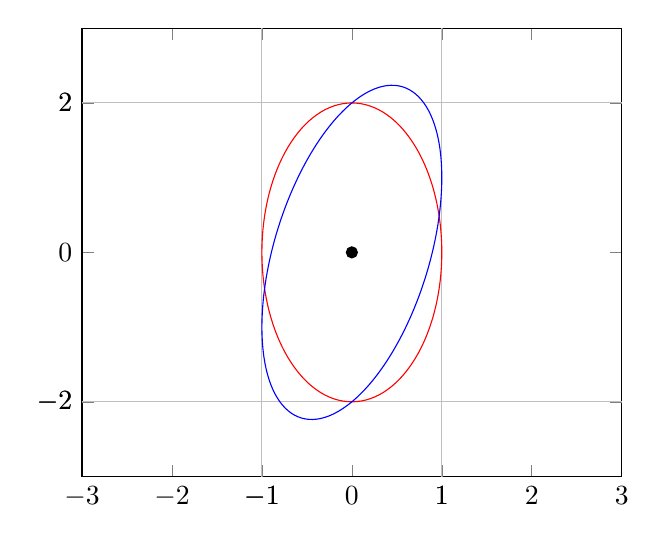
\begin{tikzpicture}
    \begin{axis}[
        xmin=-3,   xmax=3,
        ymin=-3,   ymax=3,
        extra x ticks={-1,1},
        extra y ticks={-2,2},
        extra tick style={grid=major},
    ]
        \draw[red] \pgfextra{
          \pgfpathellipse{\pgfplotspointaxisxy{0}{0}}
            {\pgfplotspointaxisdirectionxy{1}{0}}
            {\pgfplotspointaxisdirectionxy{0}{2}}
          % see also the documentation of 
          % 'axis direction cs' which
          % allows a simpler way to draw this ellipse
        };
        \draw[blue] \pgfextra{
          \pgfpathellipse{\pgfplotspointaxisxy{0}{0}}
            {\pgfplotspointaxisdirectionxy{1}{1}}
            {\pgfplotspointaxisdirectionxy{0}{2}}
        };
        \addplot [only marks,mark=*] coordinates { (0,0) };
    \end{axis}
    \end{tikzpicture}

  
  
  \begin{equation}
      x\in\mathbb{R}^{n}
  \end{equation}

  \begin{figure}[h]
    \centering
    \includegraphics[width=8cm]{pdfs/modperf/antidebug_setunhandledexceptionfilter.bson-pr.pdf}
    \caption{Example of a parametric plot ($\sin (x), \cos(x), x$)}
    \label{fig:something}
  \end{figure}

  \begin{figure}
    \centering
    \begin{subfigure}{.33\textwidth}
      \centering
      \includegraphics[width=.8\linewidth]{pdfs/modperf/antidebug_setunhandledexceptionfilter.bson-pr.pdf}
      \caption{1a}
      \label{fig:sfig1}
    \end{subfigure}%
    \begin{subfigure}{.33\textwidth}
      \centering
      \includegraphics[width=.8\linewidth]{pdfs/modperf/antidebug_setunhandledexceptionfilter.bson-roc.pdf}
      \caption{1b}
      \label{fig:sfig2}
    \end{subfigure}
    \begin{subfigure}{.33\textwidth}
        \centering
        \includegraphics[width=.8\linewidth]{pdfs/modperf/antidebug_setunhandledexceptionfilter.bson-roclog.pdf}
        \caption{1c}
        \label{fig:sfig3}
    \end{subfigure}
    \caption{plots of....}
    \label{fig:fig}
\end{figure}


\begin{table}[h]
  \centering
  \caption{This is first table}
  \begin{tabular}{@{}llr@{}} \toprule
      \multicolumn{2}{c}{Item} \\ \cmidrule(r){1-2}
      Animal & Description & Price (\$)\\ \midrule
      Gnat & per gram & 13.65 \\
      & each & 0.01 \\
      Gnu & stuffed & 92.50 \\
      Emu & stuffed & 33.33 \\
      Armadillo & frozen & 8.99 \\ \bottomrule
  \end{tabular}        
\end{table}

\begin{algorithm}
  \caption{Dependency Graph Assembly}\label{algo:AKP13_command_dependency_graph_assembly}
  \begin{algorithmic}[1]
      \Procedure{MyProcedure}{}
      \State $\textit{stringlen} \gets \text{length of }\textit{string}$
      \State $i \gets \textit{patlen}$
      \If {$i > \textit{stringlen}$} \Return false
      \EndIf
      \State $j \gets \textit{patlen}$
      \If {$\textit{string}(i) = \textit{path}(j)$}
      \State $j \gets j-1$.
      \State $i \gets i-1$.
      \State \textbf{goto} \emph{loop}.
      \State \textbf{close};
      \EndIf
      \State $i \gets i+\max(\textit{delta}_1(\textit{string}(i)),\textit{delta}_2(j))$.
      \State \textbf{goto} \emph{top}.
      \EndProcedure
  \end{algorithmic}
\end{algorithm}

\tikzset{every picture/.style={line width=0.75pt}} %set default line width to 0.75pt        

\begin{center}
    \begin{tikzpicture}[x=0.75pt,y=0.75pt,yscale=-1,xscale=1]
        %uncomment if require: \path (0,269); %set diagram left start at 0, and has height of 269
        
        %Shape: Rectangle [id:dp8386354950784081] 
        \draw   (258,67) -- (301,67) -- (301,136) -- (258,136) -- cycle ;
        %Straight Lines [id:da9088407411543793] 
        \draw    (203,103) -- (257,103) ;
        \draw [shift={(259,103)}, rotate = 180] [color={rgb, 255:red, 0; green, 0; blue, 0 }  ][line width=0.75]    (10.93,-3.29) .. controls (6.95,-1.4) and (3.31,-0.3) .. (0,0) .. controls (3.31,0.3) and (6.95,1.4) .. (10.93,3.29)   ;
        %Straight Lines [id:da7684121128470209] 
        \draw    (301,103) -- (355,103) ;
        \draw [shift={(357,103)}, rotate = 180] [color={rgb, 255:red, 0; green, 0; blue, 0 }  ][line width=0.75]    (10.93,-3.29) .. controls (6.95,-1.4) and (3.31,-0.3) .. (0,0) .. controls (3.31,0.3) and (6.95,1.4) .. (10.93,3.29)   ;
        
        % Text Node
        \draw (189,94.4) node [anchor=north west][inner sep=0.75pt]    {$x$};
        % Text Node
        \draw (274,93.4) node [anchor=north west][inner sep=0.75pt]    {$f$};
        % Text Node
        \draw (362,94.4) node [anchor=north west][inner sep=0.75pt]    {$\hat{y}$};
        
        
        \end{tikzpicture}
            
\end{center}
	

	%%%%%%%%%%%%%%%%%%%%%%%%%% 
	% APPENDIX
	\appendix	

	% \printnomenclature
	% \label{apx:nomencl}
	\chapter{Technology} \label{app:technologies}
Our technology stack is quite broad, in the lists below, we divide the tools into two groups based on what we did use it for. We do not mention standard Linux tools like \emph{shell scripts}, \emph{ssh} etc. The main part of our experimenting we spent working on Ubuntu 20.04.

In the process we usually worked with a lot of tools, we mention only those which had a significant impact in our work.


\section*{Sandboxing and infrastructure}
\subsection*{Capev2 with community signatures}
A malware sandboxing tool which provides us an environment to retrieve malware analysis which we used for further modelling. 

There are several relevant sources, here are the most important:
\begin{itemize}
  \itemsep0em 
  \item Public instance - https://capesandbox.com/
  \item Opensource project -  https://github.com/kevoreilly/CAPEv2 (under GNU General Public License v3.0)
  \item Community extensions (e.g. \ signature implementation)
  \item Documentation - https://capev2.readthedocs.io/en/latest/
\end{itemize}

\subsection*{Virtualization}
Virtualization of sandbox machines, router machine, and other related stuff was ensured by the following tools:
\begin{itemize}
  \itemsep0em 
  \item \emph{Kernel-based Virtual Machine} - https://www.linux-kvm.org
  \item \emph{VirtualBox} - https://www.virtualbox.org/
  \item \emph{Windows 7} - operating system running on sandbox virtual machines
  \item \emph{Ubuntu server} - operating system running on VPN lab edge router
  \item Other tools and sources - https://github.com/doomedraven
\end{itemize}

\subsection*{Networking}
\begin{itemize}
  \itemsep0em 
  \item Ansible - https://www.ansible.com/
  \item OpenVPN - https://openvpn.net/
  \item brctl - https://linux.die.net/man/8/brctl
  \item rsyslog - https://www.rsyslog.com/
  \item fail2ban - https://www.fail2ban.org/
  \item aide - https://aide.github.io/
  \item ufw - https://help.ubuntu.com/community/UFW
\end{itemize}

\subsection*{Programming}
For programming tasks in the infrastructure part we used \emph{Python 3} (see in \ref{app:attach}).
\subsection*{Others}
We are really pleased that we could use \emph{pafish} (https://github.com/a0rtega/pafish) as a testing malware sample, we used it many times\dots

\section*{Data and machine learning}
\subsection*{Julia}
For programming tasks in this part we used \emph{Julia} language - https://julialang.org/. Julia has many advantages regarding maily performance comparing to Python which could be considered as alternative. But we do not aspire to advocate this language, programming environment was mainly determined by the \emph{hmill} framework which is quite young and its first implementation is in this language by \cite{Mandlik2020}. List of the most important libraries used and their versions:
\begin{itemize}
  \itemsep0em 
  \item \emph{JsonGrinder.jl} - \cite{Pevny2019} (v2.1.4)
  \item \emph{Mill.jl} - \cite{Pevny2018} (v2.4.1)
  \item \emph{Flux.jl} - \cite{Innes2018a, Innes2018} (v0.11.6)
  \item \emph{EvalMetrics.jl} - https://github.com/VaclavMacha/EvalMetrics.jL (v0.2.1)
\end{itemize}
\subsection*{Computing grid system}
For resource-demanding computation we used CESNET metacenter (mentioned in acknowledgements) - https://www.metacentrum.cz/en/Sluzby/Grid/index.html.


  %-----------------------------------------
% Technology - Julia (I think I should add this in some appendix, summarize it and reference all sources used)
%   - describe why and basic features and advantages and cons
%   - Also all different codes, documented, refactored list even important libraries used in Julia

% JsonGrinder (even a little bit describe function)
% \emph{EvalMetrics.jl}

% Divide it in parts according to what we did with the infrastructure

  % Used technologies (in appendix)
%   - previous
%   - ExplainMill
%   (reference all the repositories - even cuckoo comminity)

% \todo{among appendices technologie add even (Technical background, used metascenter archicture...) and even the script
% - used technologies - add to appendix as in previous chapter
%   - \todo{reference JsonGrinder, Mill, EvalMetrics...}
%   - reference, describe functioning
% In each case, what it is, link, what we used it for
	\chapter{Trained HMILL models and their performance}
\section{Placeholder}
Hold place...

	\chapter*{Acronyms}
\begin{abbrv}
    \item[hmill]        hierarchical multiple instance learning
    \item[RAM]
    \item[JSON]
    \item[API] 
    \item[FNR] 
    \item[FPR] 
    \item[ROC] 
    \item[PRC] 
    \item[AUC] 
    \item[p.d.f.]
    \item[MLE]  
    \item[IoT] 
    \item[DDOS] 
    \item[C2 - command and control] 
    \item[HTML]
    \item[IAT]
    \item[CLI]   
    \item[GUI]
    \item[NAT]   
    \item[VPN] 
\end{abbrv}

	%Biblio
	\bibliographystyle{alpha}
	%\bibliographystyle{csplainnat}
	%bibliographystyle{plain}
	% \bibliographystyle{psc}
	%\bibliographystyle{apalike}
	{
	\bibliography{bib/Master_thesis}
	}

	% \chapter{Obsah přiloženého CD}
	% \textbf{\large Tato příloha je povinná pro každou práci. Každá práce musí totiž obsahovat přiložené CD. Viz dále.}

	% Může vypadat například takto. Váš seznam samozřejmě bude odpovídat typu vaší práce. (viz \cite{infodp}):

	% \begin{figure}[h]
	% \begin{center}
	% \includegraphics[width=14cm]{figures/seznamcd}
	% \caption{Seznam přiloženého CD --- příklad}
	% \label{fig:seznamcd}
	% \end{center}
	% \end{figure}

	% Na GNU/Linuxu si strukturu přiloženého CD můžete snadno vyrobit příkazem:\\ 
	% \verb|$ tree . >tree.txt|\\
	% Ve vzniklém souboru pak stačí pouze doplnit komentáře.

	% Z \textbf{README.TXT} (případne index.html apod.)  musí být rovněž zřejmé, jak programy instalovat, spouštět a jaké požadavky mají tyto programy na hardware.

	% Adresář \textbf{text}  musí obsahovat soubor s vlastním textem práce v PDF nebo PS formátu, který bude později použit pro prezentaci diplomové práce na WWW.

\end{document}
